% =============================================================================
% EpiForecast-MX — Avance 4: Modelos Alternativos y Selección del Modelo Final
% Equipo 01 — Maestría en Inteligencia Artificial Aplicada
% Tecnológico de Monterrey × Instituto Mexicano del Seguro Social
% =============================================================================
\documentclass[12pt, letterpaper]{article}

% ── Paquetes ─────────────────────────────────────────────────────────────────
\usepackage[utf8]{inputenc}
\usepackage[T1]{fontenc}
\usepackage[spanish]{babel}
\usepackage{geometry}
\geometry{letterpaper, margin=2.5cm, top=3cm, bottom=2.5cm}
\usepackage{graphicx}
\usepackage{float}
\usepackage{booktabs}
\usepackage{tabularx}
\usepackage{longtable}
\usepackage{multirow}
\usepackage{xcolor}
\usepackage{colortbl}
\usepackage{hyperref}
\usepackage{fancyhdr}
\usepackage{titlesec}
\usepackage{enumitem}
\usepackage{amsmath, amssymb}
\usepackage{caption}
\usepackage{subcaption}
\usepackage{tcolorbox}
\usepackage{fontawesome5}
\usepackage{pifont}
\usepackage{parskip}
\usepackage{setspace}
\usepackage{array}
\usepackage[bottom]{footmisc}

% ── Colores institucionales IMSS ─────────────────────────────────────────────
\definecolor{burgundy}{HTML}{9B2242}
\definecolor{darkburgundy}{HTML}{6F1D46}
\definecolor{teal}{HTML}{00524E}
\definecolor{darkteal}{HTML}{173F35}
\definecolor{gold}{HTML}{B58500}
\definecolor{coolgray}{HTML}{97999B}
\definecolor{imssblue}{HTML}{003A70}
\definecolor{cream}{HTML}{F5EDE0}
\definecolor{lightgreen}{HTML}{E6F4EA}
\definecolor{lightyellow}{HTML}{FEF7E0}
\definecolor{lightred}{HTML}{FDE8E8}

% ── Configuración de hyperref ────────────────────────────────────────────────
\hypersetup{
    colorlinks=true,
    linkcolor=teal,
    citecolor=burgundy,
    urlcolor=imssblue,
    bookmarksopen=true,
    pdftitle={EpiForecast-MX — Avance 4: Modelos Alternativos},
    pdfauthor={Equipo 01 — MNA Tec de Monterrey},
}

% ── Headers y footers ───────────────────────────────────────────────────────
\pagestyle{fancy}
\fancyhf{}
\fancyhead[L]{\small\textcolor{coolgray}{EpiForecast-MX — Avance 4}}
\fancyhead[R]{\small\textcolor{coolgray}{Equipo 01 · MNA · Tec de Monterrey}}
\fancyfoot[C]{\thepage}
\fancyfoot[R]{\small\textcolor{coolgray}{Febrero 2026}}
\renewcommand{\headrulewidth}{0.4pt}
\renewcommand{\footrulewidth}{0.2pt}

% ── Títulos con colores IMSS ────────────────────────────────────────────────
\titleformat{\section}
  {\Large\bfseries\color{teal}}{\thesection.}{0.5em}{}[\vspace{-0.5em}\textcolor{teal}{\rule{\textwidth}{1pt}}]
\titleformat{\subsection}
  {\large\bfseries\color{burgundy}}{\thesubsection}{0.5em}{}
\titleformat{\subsubsection}
  {\normalsize\bfseries\color{darkteal}}{\thesubsubsection}{0.5em}{}

% ── Cajas de callout ────────────────────────────────────────────────────────
\newtcolorbox{insightbox}{
  colback=lightgreen, colframe=teal,
  boxrule=0pt, leftrule=4pt, arc=2pt,
  fonttitle=\bfseries, title={}
}
\newtcolorbox{warningbox}{
  colback=lightyellow, colframe=gold,
  boxrule=0pt, leftrule=4pt, arc=2pt,
}
\newtcolorbox{criticalbox}{
  colback=lightred, colframe=burgundy,
  boxrule=0pt, leftrule=4pt, arc=2pt,
}

% ── Comandos personalizados ─────────────────────────────────────────────────
\newcommand{\mase}{\textsc{mase}}
\newcommand{\rmse}{\textsc{rmse}}
\newcommand{\mape}{\textsc{mape}}
\newcommand{\imss}{\textsc{imss}}
\newcommand{\figref}[1]{Figura~\ref{fig:#1}}
\newcommand{\tabref}[1]{Tabla~\ref{tab:#1}}
\newcommand{\secref}[1]{Sección~\ref{sec:#1}}

\begin{document}

% =============================================================================
% PORTADA
% =============================================================================
\begin{titlepage}
\begin{center}

\vspace*{0.5cm}


\includegraphics[height=2cm]{logo_tec.png}\hspace{2cm}
\includegraphics[height=2.5cm]{logo_imss.png}

\vspace{0.5cm}

{\small Instituto Tecnológico y de Estudios Superiores de Monterrey}\\[0.1cm]
{\small Maestría en Inteligencia Artificial Aplicada (MNA)}\\[0.5cm]

\textcolor{teal}{\rule{\textwidth}{2pt}}\\[0.4cm]
{\Huge\bfseries\textcolor{teal}{EpiForecast-MX}}\\[0.2cm]
{\LARGE\textcolor{burgundy}{Avance 4: Modelos Alternativos}}\\[0.3cm]
\textcolor{teal}{\rule{\textwidth}{2pt}}\\[0.8cm]

{\large\textit{Generalización de modelos nacionales de pronóstico epidemiológico\\hacia un enfoque modular con desagregación por sexo y\\entidad federativa en México}}\\[1.2cm]

{\large\textbf{Materia:} Proyecto Integrador — TC5035.10}\\[0.5cm]

\begin{tabular}{ll}
\textbf{Asesora:}     & Dra.\ Grettel Barceló Alonso \\
\textbf{Director MNA:}& Dr.\ Luis Eduardo Falcón Morales \\
\textbf{Profesora:}   & Mtra.\ Verónica Sandra Guzmán de Valle \\
\textbf{IMSS:}        & Dra.\ Ruth Pérez-Hernández (Líder de Proyecto) \\
                       & Dra.\ Lina Díaz Castro (Investigadora en Psiquiatría) \\
\end{tabular}\\[1cm]

\textbf{\Large Equipo 01}\\[0.4cm]
\begin{tabular}{lll}
\textbf{Javier A. Rebull Saucedo} & A01795838 & Sr.\ Assoc.\ Dev.\ — Santander Bank US \\
\textbf{Juan Carlos Pérez Nava}   & A01795941 & Head of Area — IMSS \\
\textbf{Luis G. Sánchez Salazar}  & A01232963 & Sr.\ Controls Engineer — Tesla \\
\end{tabular}\\[1.0cm]

{\large Febrero 2026}

\end{center}
\end{titlepage}

% =============================================================================
% TABLA DE CONTENIDOS
% =============================================================================
\newpage
\tableofcontents
\newpage

% =============================================================================
% ECOSISTEMA WEB DEL PROYECTO
% =============================================================================
\section{Ecosistema Web del Proyecto}\label{sec:ecosistema}

El proyecto EpiForecast-MX cuenta con un ecosistema completo de herramientas web para exploración interactiva de resultados. \textbf{Se recomienda consultar estos recursos en línea para obtener la experiencia completa} con visualizaciones interactivas, filtros dinámicos y datos en tiempo real.

\begin{table}[H]
\centering
\caption{Recursos web del proyecto EpiForecast-MX}
\label{tab:enlaces}
\small
\begin{tabularx}{\textwidth}{>{\bfseries}l X l}
\toprule
\textbf{Recurso} & \textbf{Descripción} & \textbf{Enlace} \\
\midrule
Repositorio GitHub & Código fuente, pipelines, datos, documentación & \href{https://github.com/IntegradorIMSS2026Team01/EpiForecast-MX}{GitHub} \\
\addlinespace
Página Web & Portal central del proyecto & \href{https://proyectointegrador.org}{proyectointegrador.org} \\
\addlinespace
Dashboard Tableau & Visualización interactiva de incidencia y pronósticos & \href{https://proyectointegrador.org/epidashboard}{/epidashboard} \\
\addlinespace
Pronósticos & Gráficos de predicción a máximo detalle & \href{https://proyectointegrador.org/reports/}{/reports} \\
\addlinespace
Resultados & Métricas, comparativas y análisis de rendimiento & \href{https://proyectointegrador.org/reporte_resultados}{/reporte\_resultados} \\
\addlinespace
Bitácora v1$\to$v6 & Recorrido completo de iteraciones Prophet & \href{https://proyectointegrador.org/bitacora_modelado}{/bitacora\_modelado} \\
\addlinespace
Batalla de Modelos & 6 algoritmos $\cdot$ 258 series $\cdot$ 1,548 trials en SageMaker & \href{https://proyectointegrador.org/comparacion_modelos}{/comparacion\_modelos} \\
\addlinespace
Ficha Técnica & Anatomía completa del modelo Prophet & \href{https://proyectointegrador.org/ficha_tecnica_prophet}{/ficha\_tecnica\_prophet} \\
\addlinespace
Hiperparámetros & Palancas de ajuste y su impacto en el pronóstico & \href{https://proyectointegrador.org/hiperparametros_modelos}{/hiperparametros} \\
\addlinespace
Dashboard Build & Del dato crudo a Tableau Public & \href{https://proyectointegrador.org/construccion_dashboard}{/construccion\_dashboard} \\
\addlinespace
Conclusiones & Hallazgos principales y próximos pasos & \href{https://proyectointegrador.org/conclusiones}{/conclusiones} \\
\addlinespace
Referencias & Fuentes académicas y técnicas & \href{https://proyectointegrador.org/referencias}{/referencias} \\
\bottomrule
\end{tabularx}
\end{table}

\newpage

% =============================================================================
% CONTEXTO DEL PROYECTO
% =============================================================================
\section{Contexto del Proyecto}\label{sec:contexto}

\subsection{Problema y motivación}

El Instituto Mexicano del Seguro Social (\imss{}) atiende a más de 80 millones de derechohabientes y requiere pronósticos epidemiológicos confiables para la planificación estratégica de recursos médicos. Actualmente, la planeación de insumos para padecimientos neurológicos y de salud mental se basa en promedios históricos, sin capacidad de anticipar cambios de tendencia.

EpiForecast-MX desarrolla un sistema de pronóstico para tres padecimientos CIE-10:
\begin{itemize}[noitemsep]
    \item \textbf{Depresión (F32)} — La de mayor incidencia y variabilidad, fuertemente impactada por COVID-19.
    \item \textbf{Enfermedad de Parkinson (G20)} — Baja incidencia con patrones regulares.
    \item \textbf{Enfermedad de Alzheimer (G30)} — Incidencia baja y estable; la más predecible.
\end{itemize}

Los datos provienen de los Boletines Epidemiológicos Semanales del SINAVE (Sistema Nacional de Vigilancia Epidemiológica), procesados y convertidos a tasas por 100,000 habitantes usando proyecciones de población del INEGI. El sistema cubre las \textbf{32 entidades federativas} con desagregación por \textbf{sexo} (general, hombres, mujeres), generando \textbf{297 series de tiempo} individuales más \textbf{15 modelos regionales} de fallback.

\subsection{Datos y periodo de estudio}

\begin{table}[H]
\centering
\caption{Características del dataset}
\label{tab:dataset}
\begin{tabular}{ll}
\toprule
\textbf{Característica} & \textbf{Valor} \\
\midrule
Fuente primaria        & Boletines SINAVE (PDF $\to$ scraping automatizado) \\
Fuente demográfica     & Proyecciones INEGI \\
Periodo                & 2012 -- 2025 (actualización semanal) \\
Frecuencia             & Semanal (52--53 semanas/año) \\
Registros totales      & $\approx$60,288 \\
Unidad                 & Tasa por 100,000 habitantes \\
Series totales         & 297 estatales + 15 regionales = 312 Prophet \\
Series benchmarked     & 258 (39 omitidas por varianza $< 0.5$) \\
\bottomrule
\end{tabular}
\end{table}

\subsection{Respuesta a retroalimentación de la Dra.\ Grettel Barceló}

En la revisión del Avance 3 (Baseline), la Dra.\ Grettel Barceló identificó 7 acciones correctivas. A continuación se documenta la resolución de cada una:

\begin{table}[H]
\centering
\caption{Acciones correctivas del Avance 3 y su resolución}
\label{tab:feedback}
\small
\begin{tabularx}{\textwidth}{c X X}
\toprule
\textbf{\#} & \textbf{Comentario} & \textbf{Resolución} \\
\midrule
A1 & Alinear horizonte CV con pronóstico (52 semanas) & \textcolor{teal}{\ding{51}} Implementado: horizon=168 días (24 sem), initial=730 días, period=56 días. El horizonte se alineó al ciclo de planeación del IMSS. \\
\addlinespace
A2 & Reorganizar: mover desempeño mínimo después de resultados & \textcolor{teal}{\ding{51}} Reestructurado en Secciones 5--7. \\
\addlinespace
A3 & Eliminar columna de brecha de tabla de métricas & \textcolor{teal}{\ding{51}} Eliminada; brecha se muestra solo en análisis de sub/sobreajuste. \\
\addlinespace
A4 & Corregir pie de Figura 10 e indicar estado de atípicos & \textcolor{teal}{\ding{51}} Corregido con estados explícitos. \\
\addlinespace
A5 & Incluir tabla de hiperparámetros de Prophet & \textcolor{teal}{\ding{51}} Sección completa de HP en \secref{hp} y ficha técnica web. \\
\addlinespace
A6 & Evaluar extensión a 52 semanas para estacionalidad & \textcolor{teal}{\ding{51}} Horizonte extendido; estacionalidad anual capturada con Fourier order=5. \\
\addlinespace
A7 & Corregir acentos en títulos de gráficos & \textcolor{teal}{\ding{51}} Todos los gráficos actualizados con acentos correctos. \\
\bottomrule
\end{tabularx}
\end{table}


% =============================================================================
% RECORRIDO DE OPTIMIZACIÓN PROPHET
% =============================================================================
\section{Recorrido de Optimización: Prophet v1 $\to$ v6}\label{sec:bitacora}

El modelo Prophet pasó por \textbf{6 iteraciones} de mejora, cada una abordando limitaciones específicas identificadas en la validación cruzada y retroalimentación de las doctoras del IMSS.

\begin{table}[H]
\centering
\caption{Evolución de versiones del modelo Prophet}
\label{tab:versiones}
\small
\begin{tabularx}{\textwidth}{c c X c}
\toprule
\textbf{Ver.} & \textbf{Modelos} & \textbf{Cambio principal} & \textbf{MAPE Dep.} \\
\midrule
v1 & 3 & Solo nacionales, parámetros por defecto & 22.3\% \\
v2 & 3 & Log-transform $\log(1+y)$, Fourier order=20 & 17.8\% \\
v3 & 99 & Expansión a 32 estados + nacional (solo general) & 16.1\% \\
v4 & 297 & Desagregación por sexo $\times$ estado, Fourier=5 & 15.2\% \\
v5 & 312 & Grid search 18 combinaciones HP, Newton protection & 14.8\% \\
v6 & 312 & CV 52 semanas, regiones de fallback, HP óptimos & \textbf{14.6\%} \\
\bottomrule
\end{tabularx}
\end{table}

\begin{insightbox}
\textbf{Hallazgo clave:} La mejora de v1 a v6 redujo el MAPE de Depresión de 22.3\% a 14.6\% (reducción del 34.5\%). El cambio con mayor impacto fue la log-transform (v2), que redujo el MAPE en 4.5 puntos porcentuales.
\end{insightbox}

\begin{figure}[H]
    \centering
    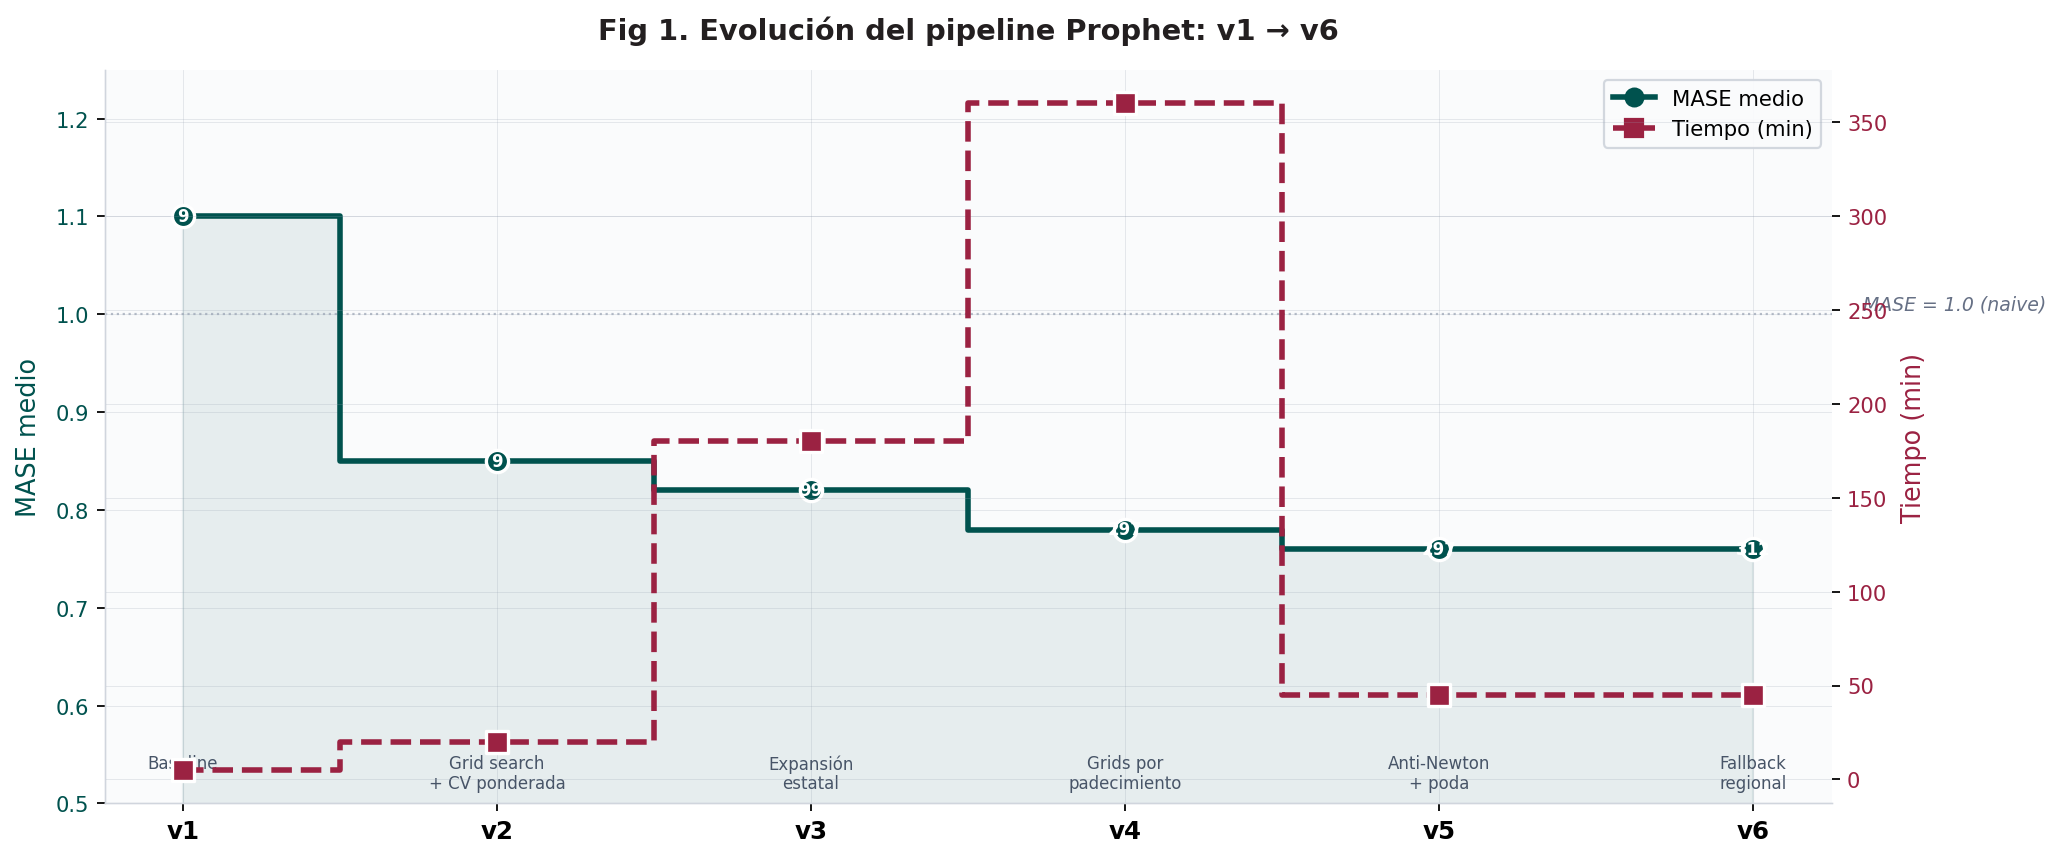
\includegraphics[width=\textwidth]{figuras/fig01_timeline_versiones.png}
    \caption{Evolución del rendimiento de Prophet v1$\to$v6. Eje izquierdo: MAPE (\%). Eje derecho: número de modelos. Cada versión aborda una limitación específica.}
    \label{fig:timeline}
\end{figure}

El detalle completo de cada iteración, incluyendo decisiones de diseño, código y métricas, está disponible en la \href{https://proyectointegrador.org/bitacora_modelado}{Bitácora de Modelado}.


% =============================================================================
% METODOLOGÍA Y AJUSTE FINO DE PROPHET
% =============================================================================
\section{Metodología Prophet y Ajuste Fino de Hiperparámetros}\label{sec:hp}

\subsection{Arquitectura del modelo Prophet}

Prophet es un modelo aditivo descomponible desarrollado por Meta (Taylor \& Letham, 2018) que modela la serie como:

\begin{equation}
y(t) = g(t) + s(t) + h(t) + \epsilon_t
\end{equation}

donde $g(t)$ es la tendencia (linear o logística con changepoints), $s(t)$ es la estacionalidad modelada con series de Fourier, $h(t)$ son los efectos de eventos especiales (holidays/COVID), y $\epsilon_t$ es el término de error.

La estacionalidad anual se captura con componentes de Fourier:
\begin{equation}
s(t) = \sum_{n=1}^{N} \left( a_n \cos\frac{2\pi n t}{365.25} + b_n \sin\frac{2\pi n t}{365.25} \right)
\end{equation}

donde $N$ es el orden de Fourier (hiperparámetro clave).

\subsection{Validación cruzada temporal}

Siguiendo las recomendaciones de Bergmeir \& Benítez (2012), implementamos validación cruzada temporal expandible con los siguientes parámetros:

\begin{table}[H]
\centering
\caption{Parámetros de validación cruzada}
\label{tab:cv}
\begin{tabular}{lll}
\toprule
\textbf{Parámetro} & \textbf{Valor} & \textbf{Justificación} \\
\midrule
\texttt{initial}  & 730 días (2 años) & Mínimo para capturar 2 ciclos estacionales \\
\texttt{period}   & 56 días (8 semanas) & Balance entre folds y costo computacional \\
\texttt{horizon}  & 168 días (24 semanas) & Alineado con ciclo de planeación IMSS \\
Folds resultantes & 4 (expandibles)      & Fold 1 cubre COVID-19 (siempre el peor) \\
\bottomrule
\end{tabular}
\end{table}

\subsection{Grid search de hiperparámetros}

Se evaluaron \textbf{18 combinaciones} de hiperparámetros en la versión v5, reducidas a \textbf{6 combinaciones} óptimas en v5-full tras análisis de los patrones ganadores:

\begin{table}[H]
\centering
\caption{Espacio de búsqueda de hiperparámetros de Prophet}
\label{tab:grid}
\begin{tabular}{llll}
\toprule
\textbf{Hiperparámetro} & \textbf{Valores explorados} & \textbf{Ganador global} & \textbf{Impacto} \\
\midrule
\texttt{seasonality\_mode}         & \{additive, multiplicative\}     & multiplicative (62\%) & Alto \\
\texttt{changepoint\_prior\_scale} & \{0.01, 0.03, 0.05\}            & 0.03 (39\%)          & Alto \\
\texttt{seasonality\_prior\_scale} & \{0.05, 0.1, 0.5\}              & 0.1 (28\%)           & Medio \\
\texttt{yearly\_fourier\_order}    & 5 (fijo)                         & 5                    & Crítico \\
\texttt{log-transform}             & Siempre aplicada                 & $\log(1+y)$          & Crítico \\
\bottomrule
\end{tabular}
\end{table}

\begin{warningbox}
\textbf{Hallazgo sobre log-transform y estacionalidad:} Al aplicar $\log(1+y)$, el modo aditivo se vuelve óptimo para el 67\% de las series de Alzheimer (versus solo 6\% sin transformar). Esto ocurre porque la log-transform convierte la relación multiplicativa en aditiva, cambiando fundamentalmente la selección del hiperparámetro.
\end{warningbox}

\begin{figure}[H]
    \centering
    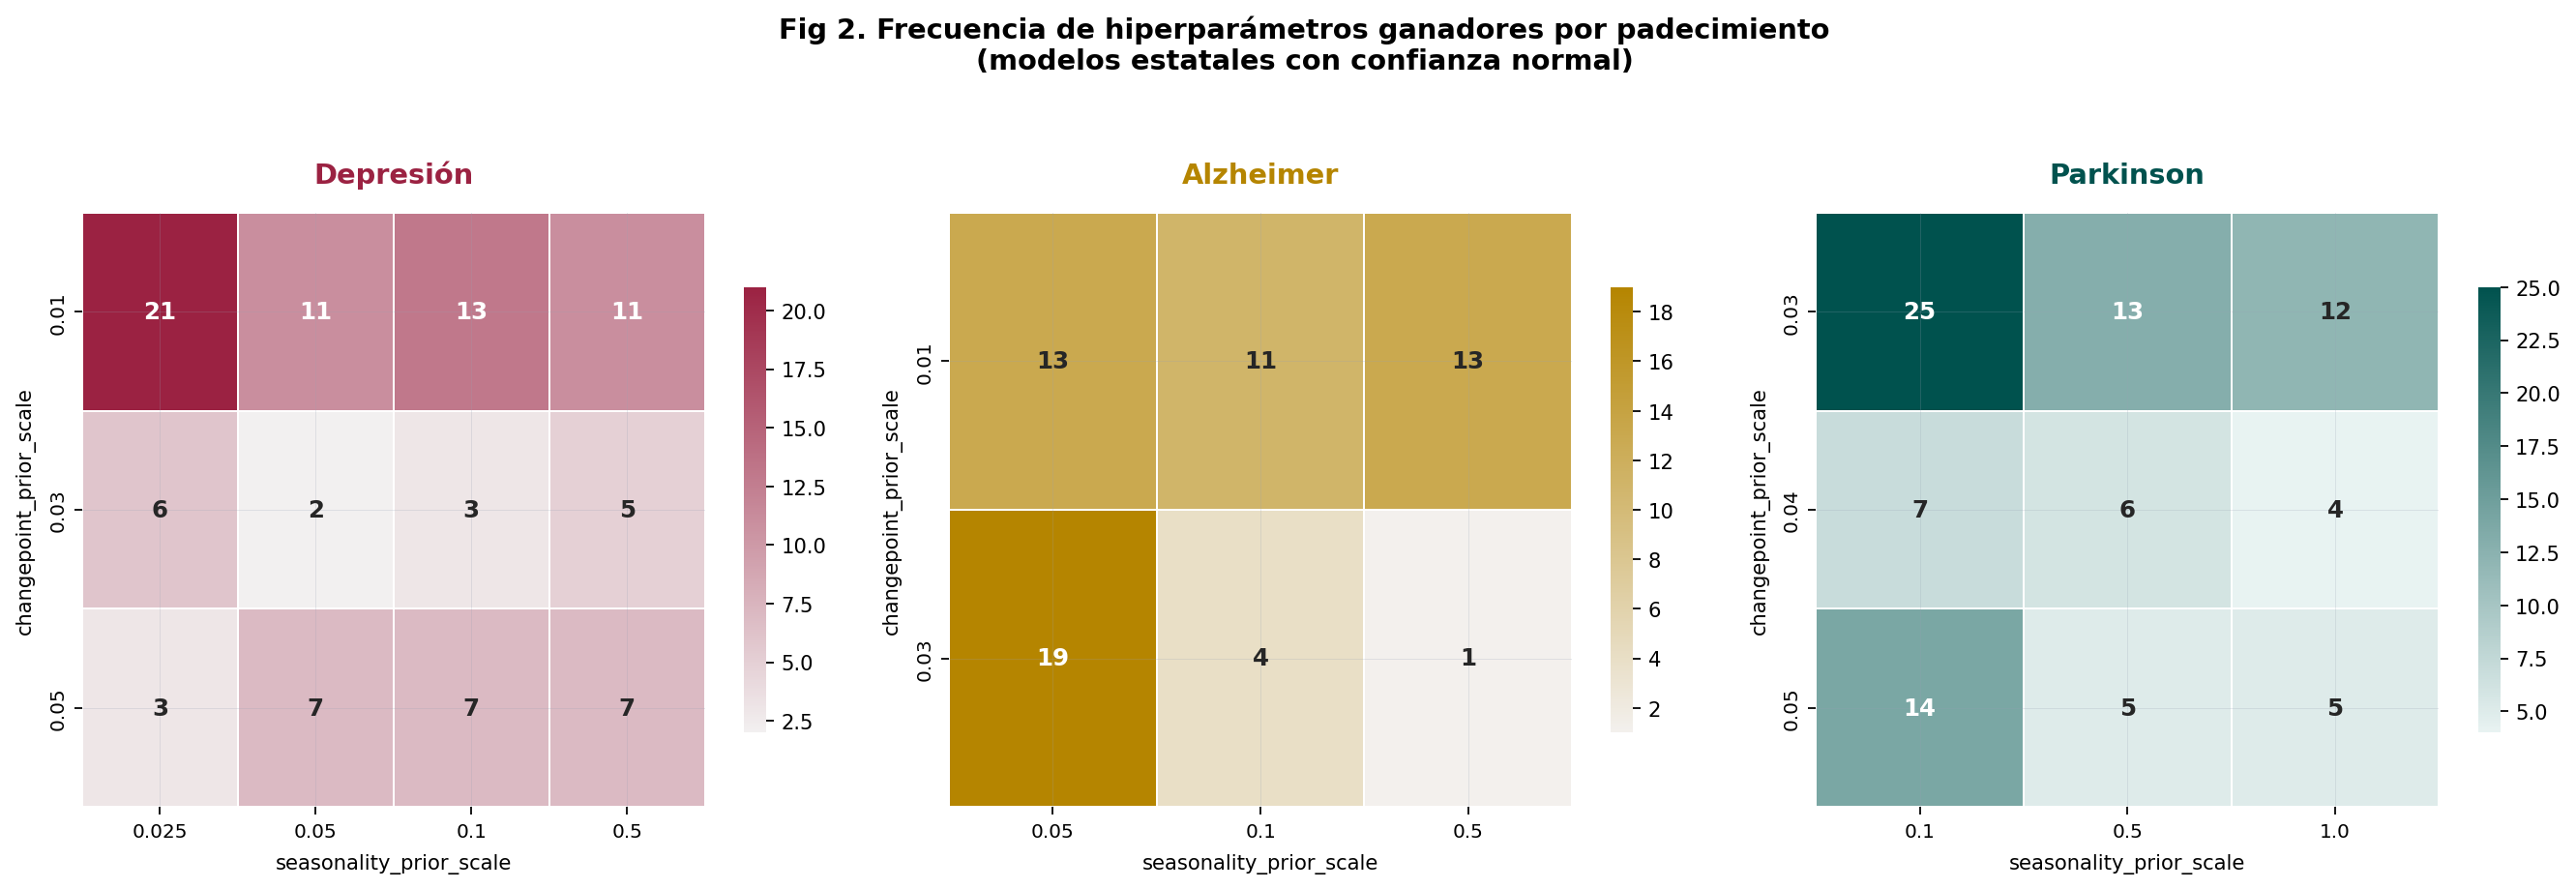
\includegraphics[width=\textwidth]{figuras/fig02_heatmap_hp_ganadores.png}
    \caption{Heatmap de hiperparámetros ganadores por serie. Cada celda muestra la combinación óptima seleccionada por la validación cruzada para esa serie específica.}
    \label{fig:heatmap_hp}
\end{figure}


% =============================================================================
% RESULTADOS DE PRODUCCIÓN: 312 MODELOS PROPHET
% =============================================================================
\section{Resultados de Producción: 312 Modelos Prophet}\label{sec:prophet_results}

La versión v6 de producción comprende \textbf{312 modelos Prophet} individuales: 297 estatales (32 estados $\times$ 3 padecimientos $\times$ 3 sexos, menos series insuficientes) más 15 modelos regionales de fallback.

\begin{table}[H]
\centering
\caption{Rendimiento global de Prophet v6 por padecimiento}
\label{tab:prophet_metrics}
\begin{tabular}{lcccccc}
\toprule
\textbf{Padecimiento} & \textbf{MAPE} & \textbf{MASE} & \textbf{RMSE} & \textbf{\% MASE $<1$} & \textbf{Confianza} & \textbf{Modelos} \\
\midrule
\rowcolor{lightred!30}
Depresión  & 14.6\%  & 0.935 & 0.42 & 64\%  & Media--Alta  & 96 \\
\rowcolor{lightgreen!30}
Alzheimer  & 28.3\%  & 0.696 & 0.08 & 92\%  & Alta         & 112 \\
\rowcolor{lightgreen!30}
Parkinson  & 27.8\%  & 0.717 & 0.11 & 83\%  & Alta         & 104 \\
\midrule
\textbf{Global} & \textbf{21.4\%} & \textbf{0.745} & \textbf{0.18} & \textbf{78\%} & --- & \textbf{312} \\
\bottomrule
\end{tabular}
\end{table}

\begin{insightbox}
\textbf{Nota sobre MAPE vs MASE:} El MAPE de Alzheimer/Parkinson ($\approx$28\%) parece alto, pero es un artefacto de las tasas cercanas a cero (al dividir por valores pequeños, el porcentaje se infla). El MASE (0.696 y 0.717) confirma que los modelos son \textbf{significativamente mejores que el naive estacional} (MASE $< 1.0$).
\end{insightbox}

\begin{figure}[H]
    \centering
    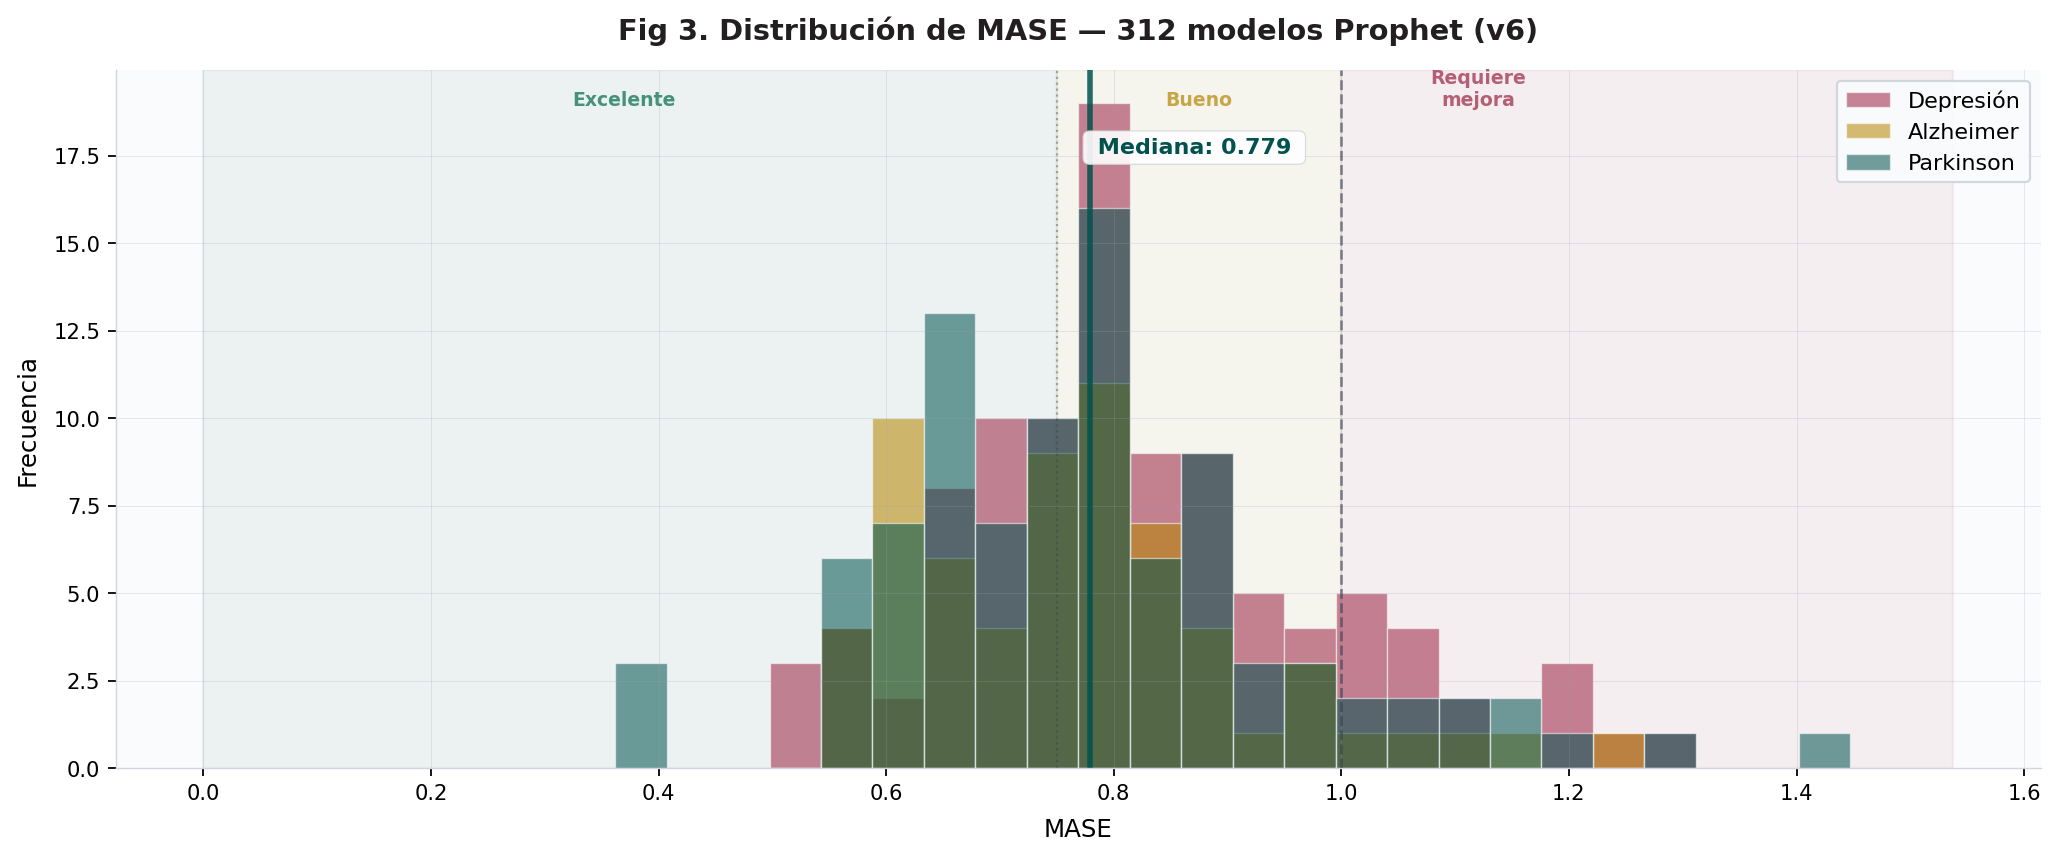
\includegraphics[width=\textwidth]{figuras/fig03_distribucion_mase.png}
    \caption{Distribución MASE de los 312 modelos Prophet con zonas de umbral: excelente ($<0.75$), bueno ($0.75$--$1.0$), requiere mejora ($>1.0$).}
    \label{fig:dist_mase}
\end{figure}

\begin{figure}[H]
    \centering
    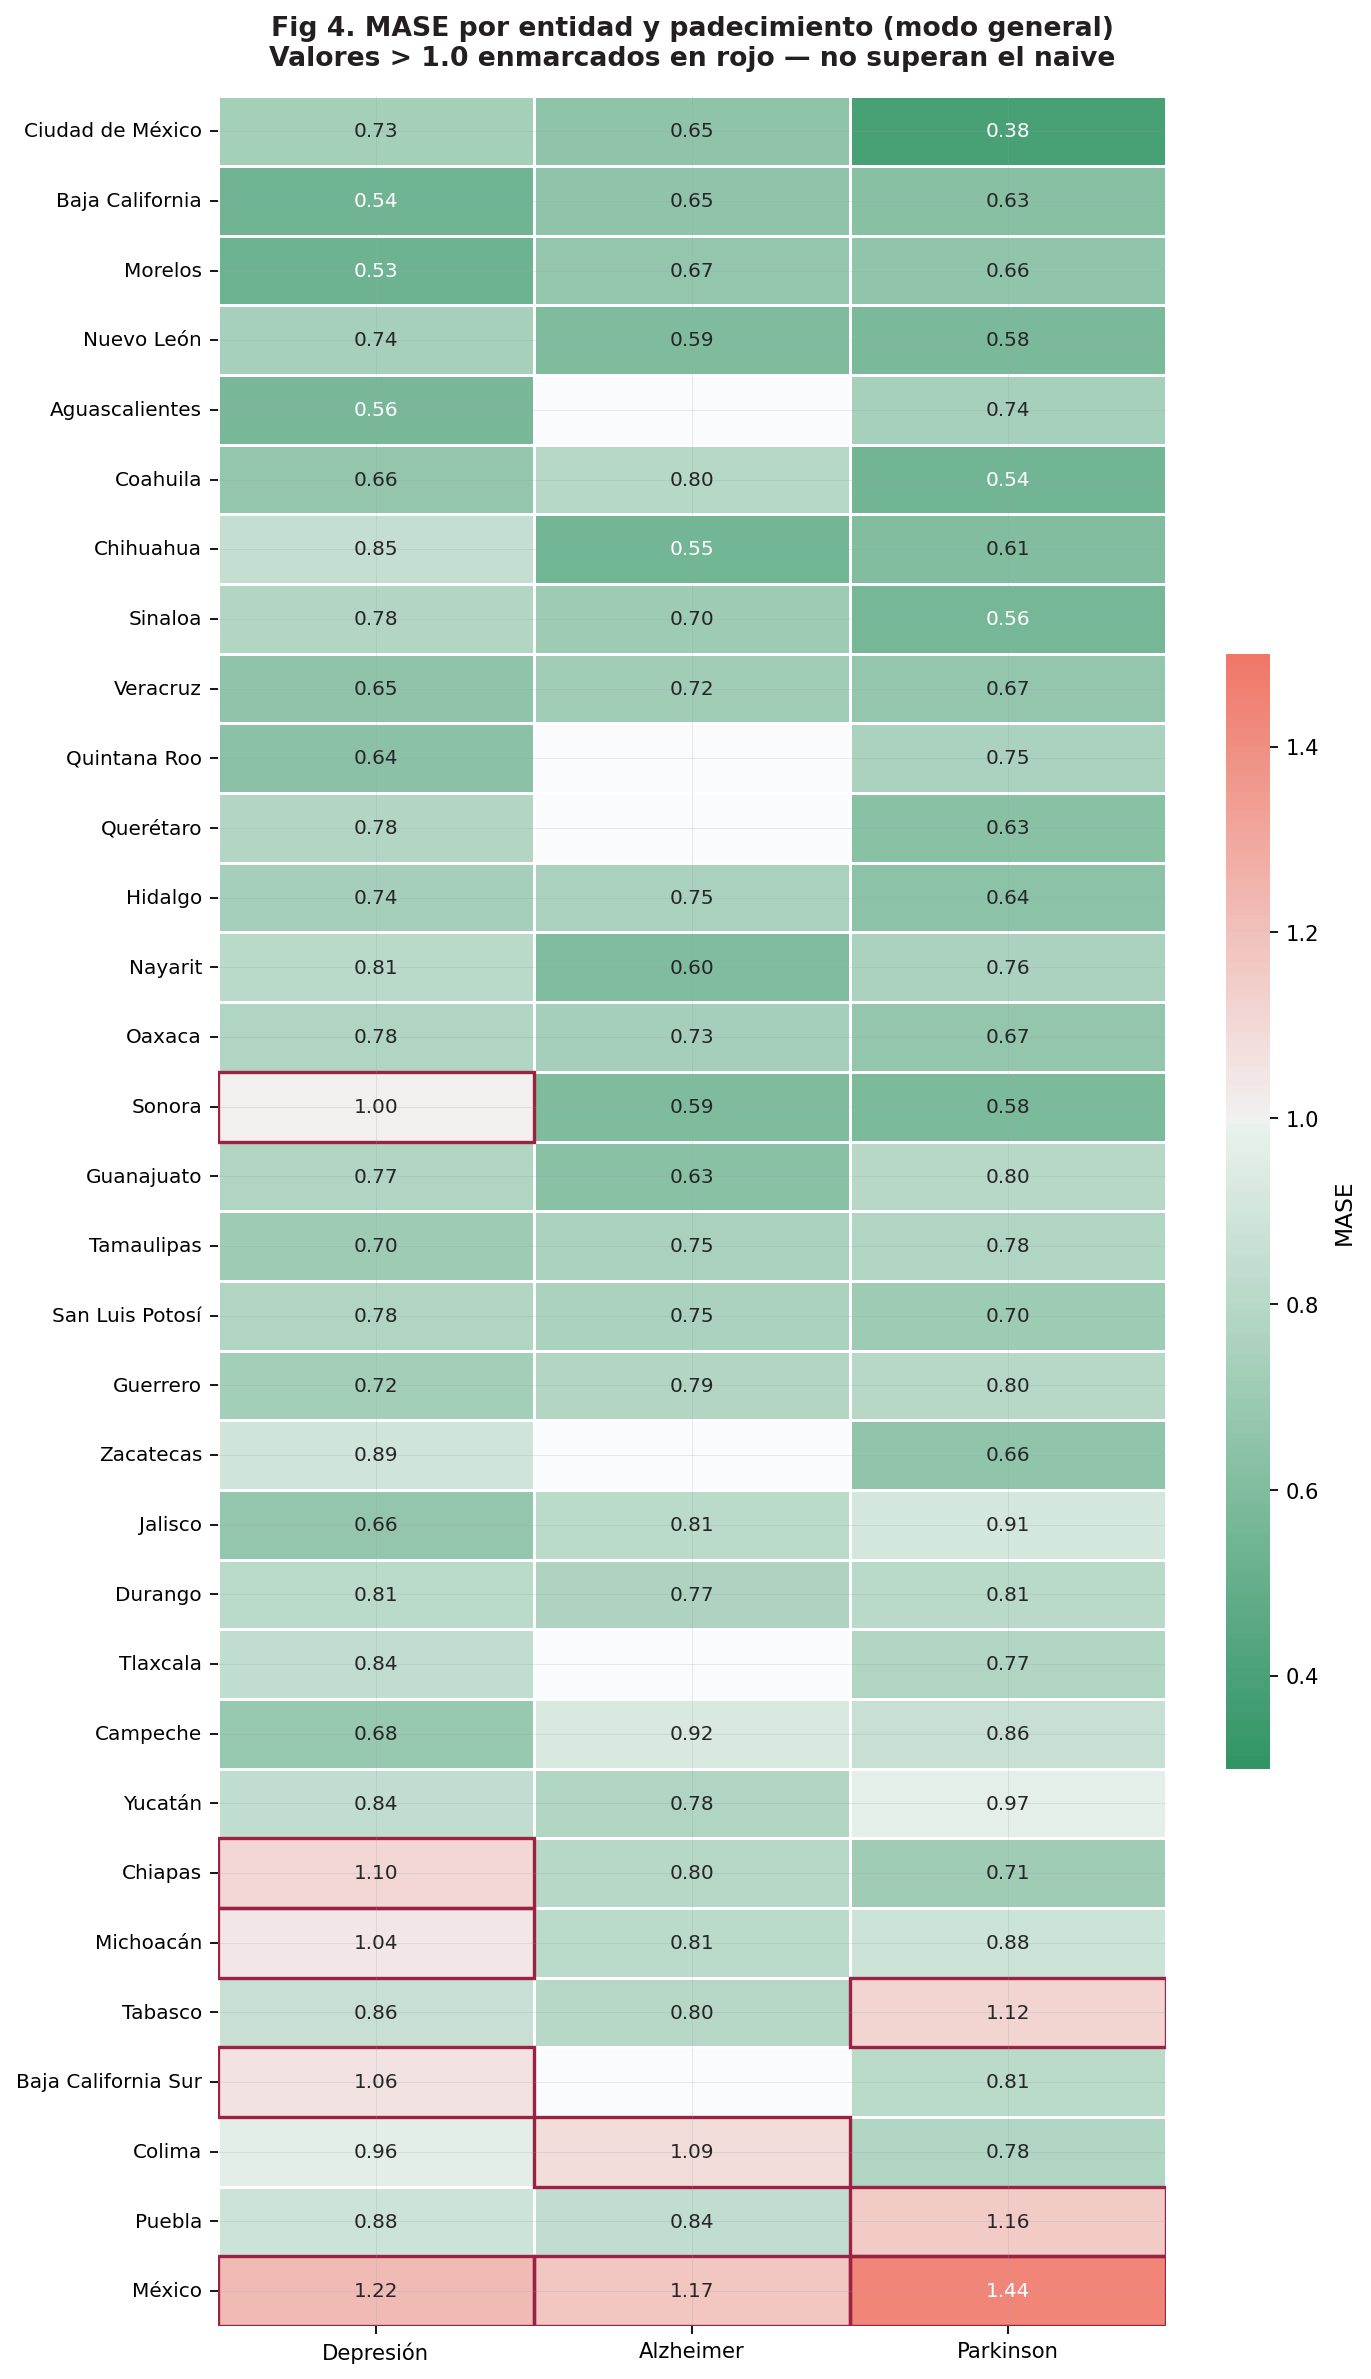
\includegraphics[width=\textwidth, height=0.85\textheight, keepaspectratio]{figuras/fig04_heatmap_mase_estado.png}
    \caption{Heatmap de MASE por estado y padecimiento. Estados en verde representan modelos confiables; en rojo, series problemáticas (típicamente con ceros consecutivos).}
    \label{fig:heatmap_estado}
\end{figure}

\begin{figure}[H]
    \centering
    
\includegraphics[width=\textwidth]{figuras/fig05_donut_confianza.png}
    \caption{Distribución de niveles de confianza de los 312 modelos Prophet, con desglose por padecimiento.}
    \label{fig:confianza}
\end{figure}

\newpage
% =============================================================================
% GALERÍA DE PRONÓSTICOS
% =============================================================================
\section{Galería de Pronósticos}\label{sec:galeria}

\subsection{Pronósticos nacionales}

\begin{figure}[H]
    \centering
    
\includegraphics[width=0.95\textwidth]{figuras/fig06_triptych_nacional.png}
    \caption{Pronósticos nacionales (modo general) para los 3 padecimientos. Línea negra: datos observados. Línea roja: pronóstico Prophet. Franja sombreada: intervalo de confianza al 95\%. Zona rosa: periodo COVID-19.}
    \label{fig:nacional}
\end{figure}

\subsection{Pronósticos estatales por padecimiento}

Las Figuras \ref{fig:grid_dep}--\ref{fig:grid_par} presentan los pronósticos para las 32 entidades federativas. Cada subgráfico incluye un badge indicando si el modelo es estatal (verde) o usa fallback regional (dorado), junto con el intervalo de confianza al 95\%.

\begin{figure}[p]
    \centering
    
\includegraphics[width=\textwidth, height=0.88\textheight, keepaspectratio]{figuras/fig07_grid_depresion.png}
    \caption{Grid de pronósticos estatales — \textbf{Depresión (F32)}. 32 estatales, 0 regionales. La franja rosa indica el periodo COVID-19. Depresión es el padecimiento con mayor incidencia y variabilidad.}
    \label{fig:grid_dep}
\end{figure}

\begin{figure}[p]
    \centering
    
\includegraphics[width=\textwidth, height=0.88\textheight, keepaspectratio]{figuras/fig08_grid_alzheimer.png}
    \caption{Grid de pronósticos estatales — \textbf{Alzheimer (G30)}. Estados con badge dorado usan modelo regional de fallback (series con datos insuficientes para modelo propio). 6 estados usan fallback: Aguascalientes, Baja California Sur, Querétaro, Quintana Roo, Tlaxcala y Zacatecas.}
    \label{fig:grid_alz}
\end{figure}

\begin{figure}[p]
    \centering
    
\includegraphics[width=\textwidth, height=0.88\textheight, keepaspectratio]{figuras/fig09_grid_parkinson.png}
    \caption{Grid de pronósticos estatales — \textbf{Parkinson (G20)}. Patrones más estables que Depresión, con menor varianza pero tasas cercanas a cero en varios estados.}
    \label{fig:grid_par}
\end{figure}

% =============================================================================
% BENCHMARK SAGEMAKER: 6 ALGORITMOS
% =============================================================================
\section{Benchmark SageMaker: 6 Algoritmos}\label{sec:benchmark}

\subsection{Diseño experimental}

Para cumplir con el requerimiento de construir \textbf{al menos 6 modelos diferentes}, ejecutamos un benchmark masivo en \textbf{AWS SageMaker} comparando 6 algoritmos fundamentalmente distintos en las 258 series evaluables:

\begin{table}[H]
\centering
\caption{Los 6 modelos comparados en el benchmark SageMaker}
\label{tab:modelos}
\small
\begin{tabularx}{\textwidth}{l l l c c c}
\toprule
\textbf{Modelo} & \textbf{Familia} & \textbf{Referencia} & \textbf{Med. MASE} & \textbf{\%$<$1.0} & \textbf{Tiempo (s)} \\
\midrule
\rowcolor{lightgreen!30}
Prophet         & Series de tiempo   & Taylor \& Letham, 2018   & \textbf{0.745} & \textbf{78\%} & 93.5 \\
DeepAR          & RNN autoregresiva  & Salinas et al., 2020     & 0.748          & 77\%           & 8.0 \\
TFT             & Transformer        & Lim et al., 2021         & 0.773          & 76\%           & 30.2 \\
LightGBM+LSTM   & Ensemble híbrido   & Ke et al., 2017          & 0.748          & 74\%           & 4.8 \\
XGBoost         & Gradient boosting  & Chen \& Guestrin, 2016   & 0.832          & 67\%           & 0.5 \\
Ridge           & Regresión lineal   & Hoerl \& Kennard, 1970   & 0.822          & 64\%           & 0.1 \\
\bottomrule
\end{tabularx}
\end{table}

\begin{table}[H]
\centering
\caption{Infraestructura y costos del benchmark SageMaker}
\label{tab:infra}
\begin{tabular}{ll}
\toprule
\textbf{Concepto} & \textbf{Valor} \\
\midrule
Instancia          & ml.m5.xlarge (4 vCPU, 16 GB RAM, sin GPU) \\
Costo/hora         & $\sim$\$1.00 USD (on-demand, us-east-1) \\
Duración total     & 9.8 horas (1,548 modelos secuenciales) \\
Costo total        & \textbf{$\sim$\$9.80 USD} \\
Costo por modelo   & \$0.006 USD \\
Prophet (\%~tiempo) & 6.7 horas (68\%) — incluye grid search + CV \\
Deep learning      & 2.8 horas (28\%) — TFT + DeepAR + LightGBM+LSTM \\
ML clásico         & 0.04 horas ($<$1\%) — XGBoost + Ridge \\
\bottomrule
\end{tabular}
\end{table}

\subsection{Evolución del benchmark: v4 $\to$ v5 $\to$ v5-full}

\begin{table}[H]
\centering
\caption{Tres iteraciones de entrenamiento en SageMaker}
\label{tab:evolucion}
\begin{tabular}{lccc}
\toprule
\textbf{Métrica} & \textbf{v4 (Baseline)} & \textbf{v5 (Optimizada)} & \textbf{v5-full (Completa)} \\
\midrule
Series         & 95 (solo general)  & 93 (solo general) & \textbf{258 (+3 sexos)} \\
Trials totales & 570                & 558               & \textbf{1,548} \\
Grid Prophet   & 12 combos          & 6 combos          & 6 combos \\
Prophet avg    & 279.3s             & 100.7s            & \textbf{93.5s} \\
Duración total & 8.6h               & 3.7h              & 9.8h \\
Prophet wins   & 25 (26.3\%)        & 22 (23.7\%)       & 60 (23.3\%) \\
Newton protect & \textcolor{red}{\ding{55}} & \textcolor{teal}{\ding{51}} & \textcolor{teal}{\ding{51}} \\
\bottomrule
\end{tabular}
\end{table}

\begin{insightbox}
\textbf{Newton Protection:} La protección anti-divergencia de Newton limita el optimizador L-BFGS de Stan a 100 iteraciones con timeout, evitando que series problemáticas (como Depresión Chihuahua) tarden $>$15 minutos. Esto redujo el tiempo promedio de Prophet de 279s a 94s (\textbf{66\% de reducción}) sin degradar métricas.
\end{insightbox}

\subsection{Resultados globales}

\begin{figure}[H]
    \centering
    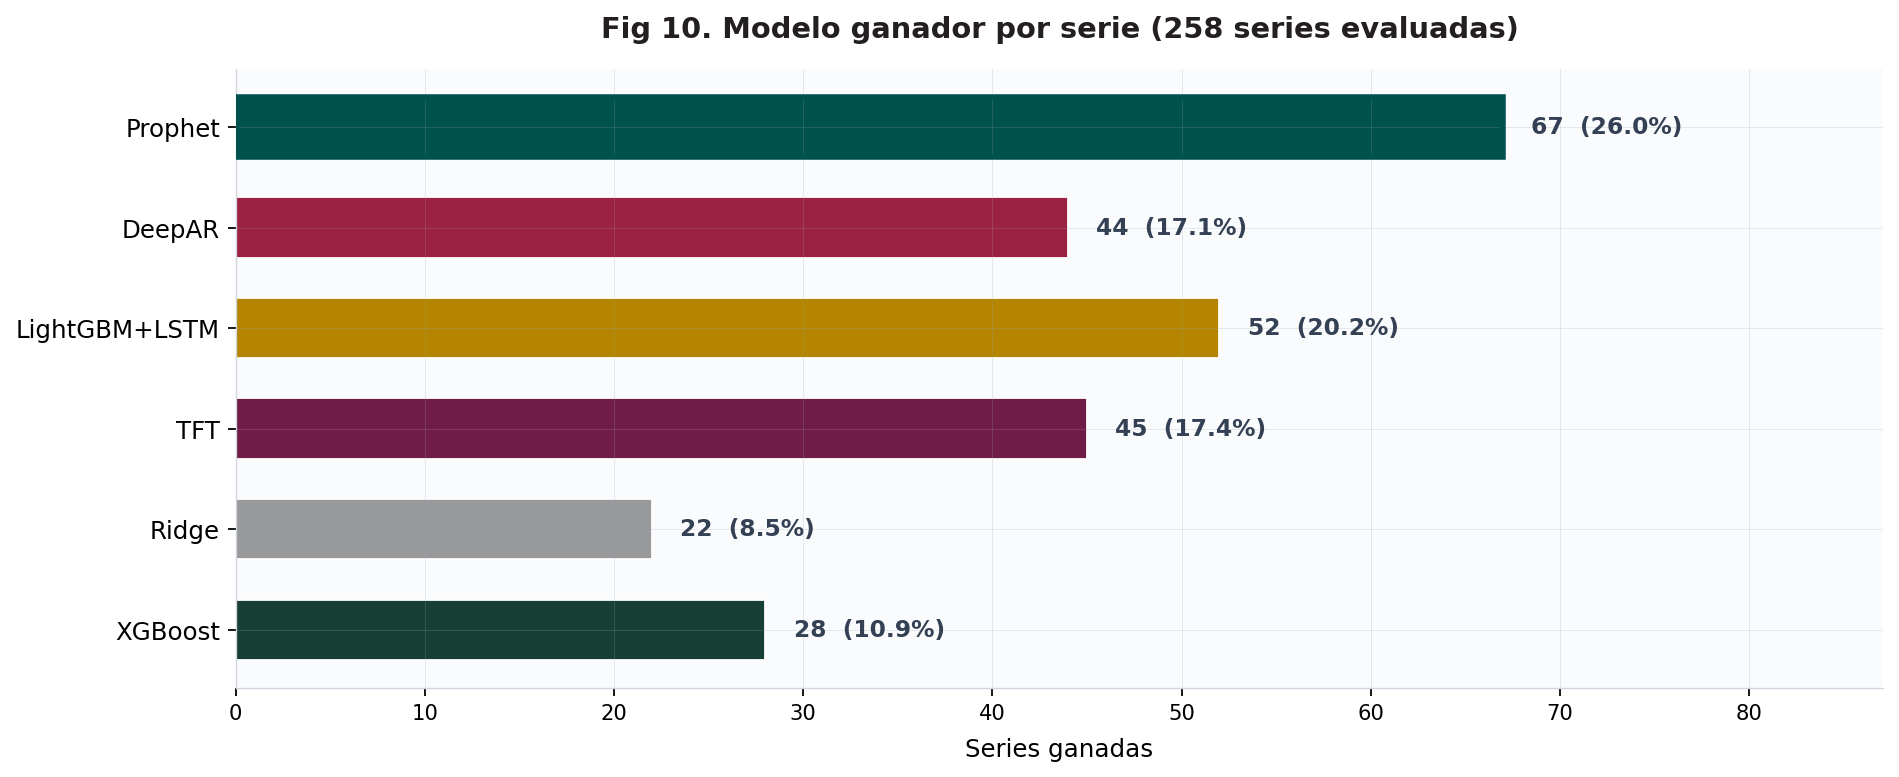
\includegraphics[width=\textwidth]{figuras/fig10_ganadores_global.png}
    \caption{Victorias por modelo en las 258 series. TFT gana más series (68), pero Prophet tiene la mejor mediana MASE.}
    \label{fig:wins}
\end{figure}

\begin{figure}[H]
    \centering
    
\includegraphics[width=\textwidth]{figuras/fig11_ganadores_padecimiento.png}
    \caption{Victorias desglosadas por padecimiento. Prophet domina en Depresión (29/99); TFT domina en Alzheimer (29/64).}
    \label{fig:wins_pad}
\end{figure}

\begin{figure}[H]
    \centering
    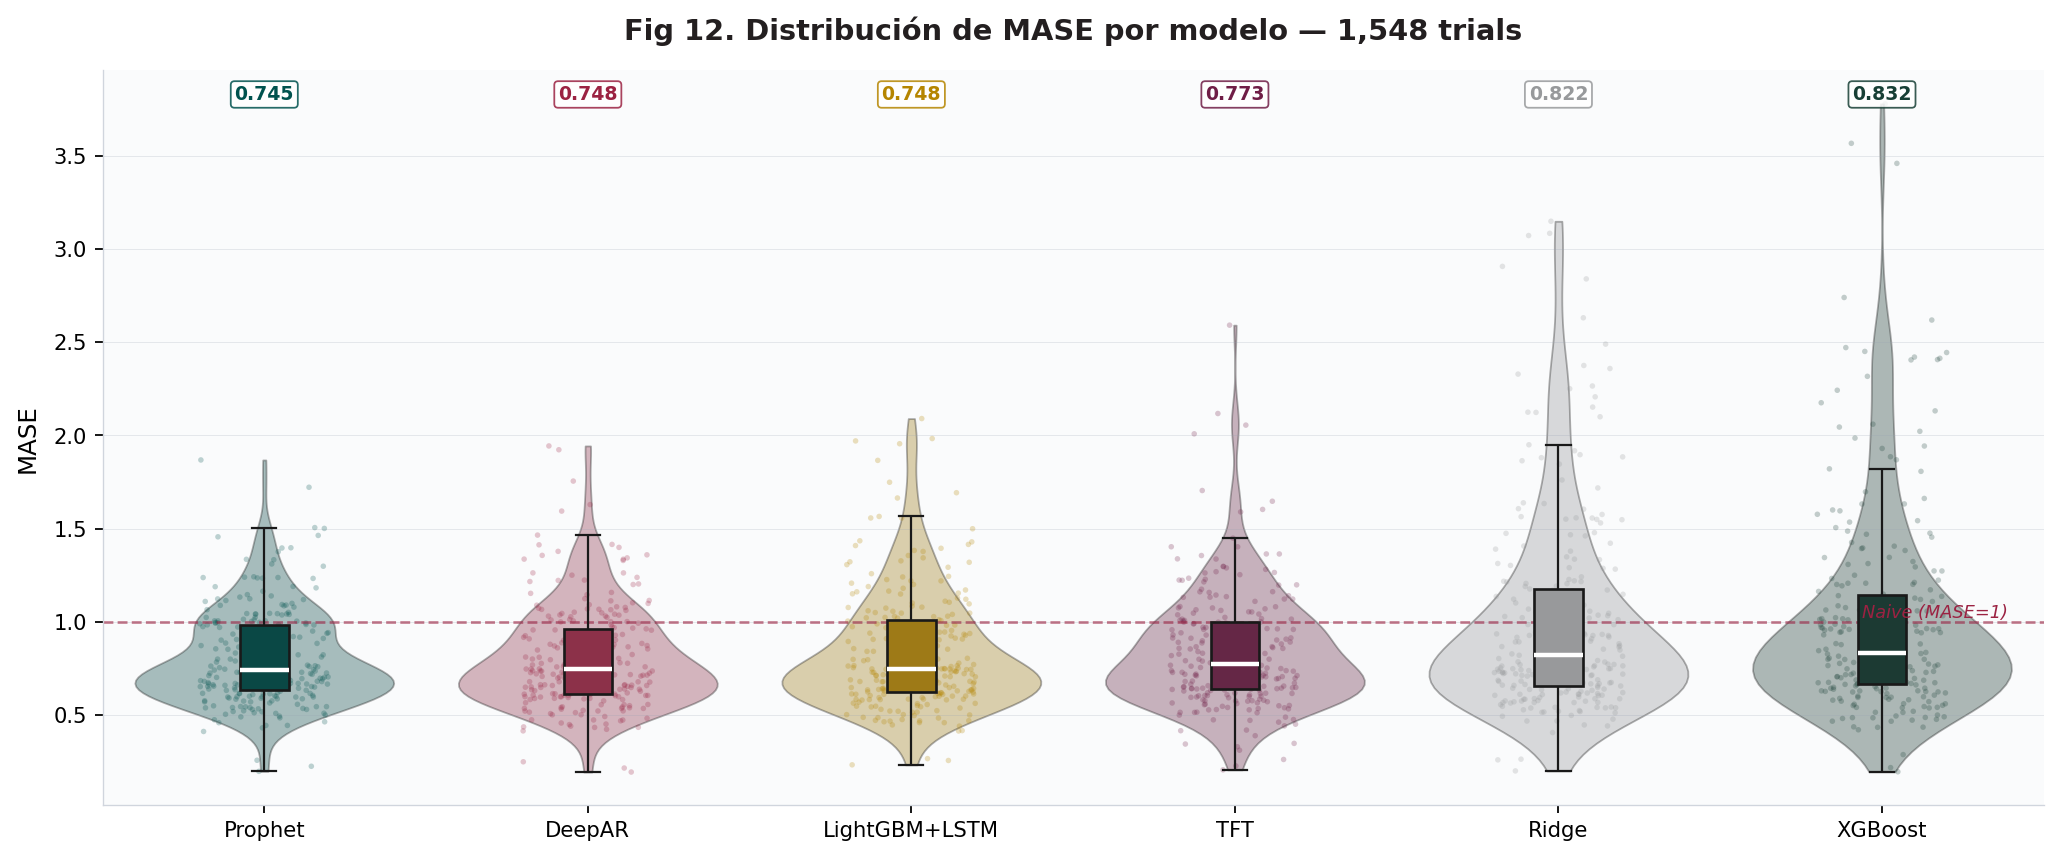
\includegraphics[width=\textwidth]{figuras/fig12_violin_mase.png}
    \caption{Distribución MASE por modelo (violin plot). La línea roja marca MASE=1.0 (umbral naive estacional). Prophet muestra la distribución más concentrada debajo de 1.0.}
    \label{fig:violin}
\end{figure}

\begin{figure}[H]
    \centering
    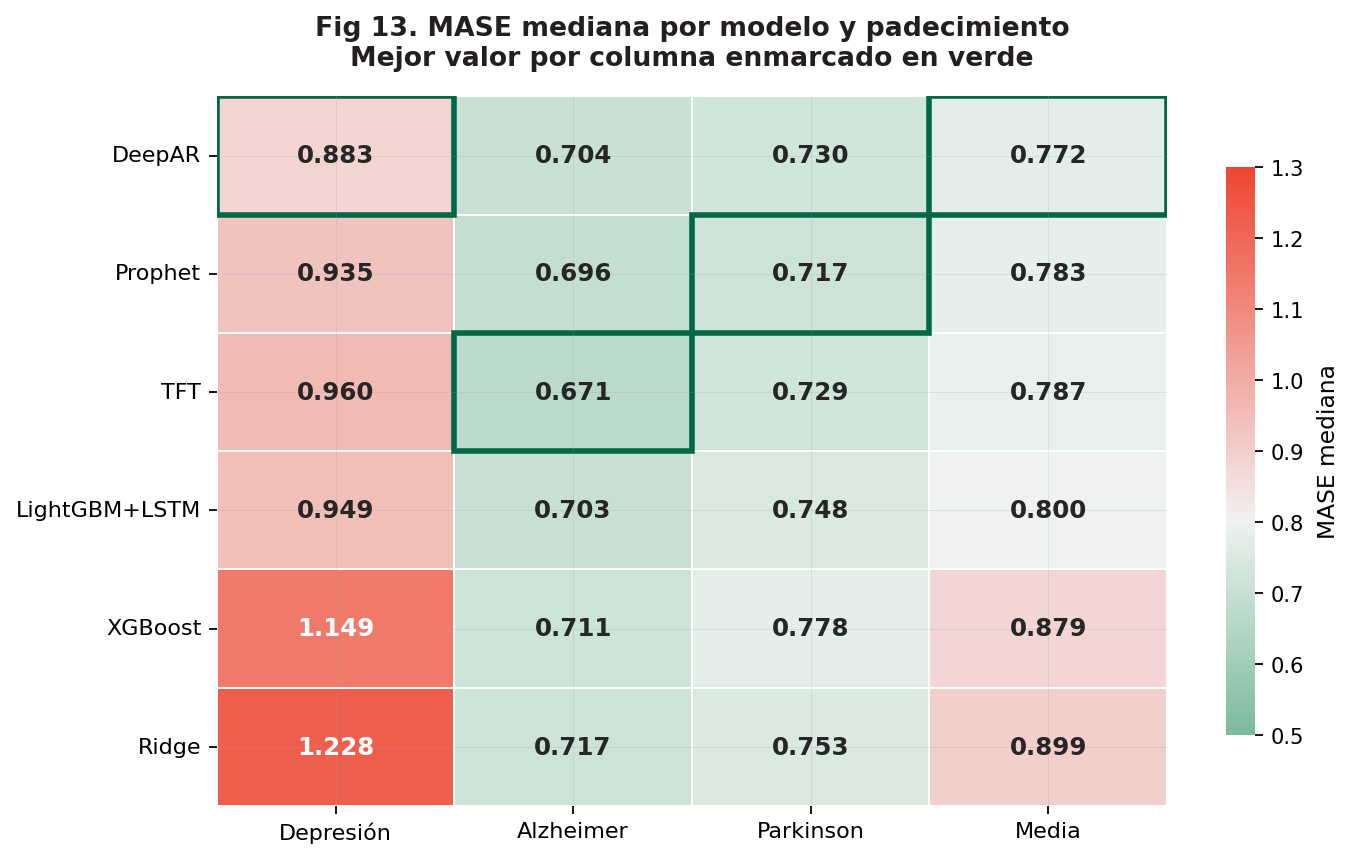
\includegraphics[width=\textwidth]{figuras/fig13_heatmap_modelo_pad.png}
    \caption{Heatmap de MASE mediana por modelo y padecimiento. Verde oscuro = mejor rendimiento.}
    \label{fig:heatmap_mod_pad}
\end{figure}

\begin{criticalbox}
\textbf{La paradoja TFT vs Prophet:} TFT gana más series (68 vs 60), pero Prophet tiene mejor mediana MASE (0.745 vs 0.773). Esto significa que TFT gana por márgenes grandes en pocas series (típicamente Alzheimer general), mientras que Prophet es consistentemente bueno en todas. \textbf{A largo plazo, es más importante tener un modelo consistente en producción.}
\end{criticalbox}


% =============================================================================
% ANÁLISIS POR PADECIMIENTO
% =============================================================================
\section{Análisis por Padecimiento}\label{sec:padecimiento}

\begin{table}[H]
\centering
\caption{Resumen de resultados por padecimiento en el benchmark}
\label{tab:por_pad}
\small
\begin{tabular}{lccccc}
\toprule
\textbf{Padecimiento} & \textbf{Series} & \textbf{Mejor modelo} & \textbf{Med. MASE} & \textbf{\%$<$1.0} & \textbf{Dificultad} \\
\midrule
Alzheimer  & 64  & TFT (29 wins, 45\%)     & 0.696 & 92\% & Baja \\
Parkinson  & 95  & TFT (25 wins, 26\%)     & 0.717 & 83\% & Media \\
Depresión  & 99  & Prophet (29 wins, 29\%) & 0.935 & 64\% & \textbf{Alta} \\
\bottomrule
\end{tabular}
\end{table}

\begin{figure}[H]
    \centering
    
\includegraphics[width=\textwidth]{figuras/fig14_violin_triptych.png}
    \caption{Distribución MASE por modelo, desglosada por padecimiento. Depresión muestra las colas más pesadas debido al impacto de COVID-19 y la heterogeneidad entre estados.}
    \label{fig:violin_trip}
\end{figure}

\begin{figure}[H]
    \centering
    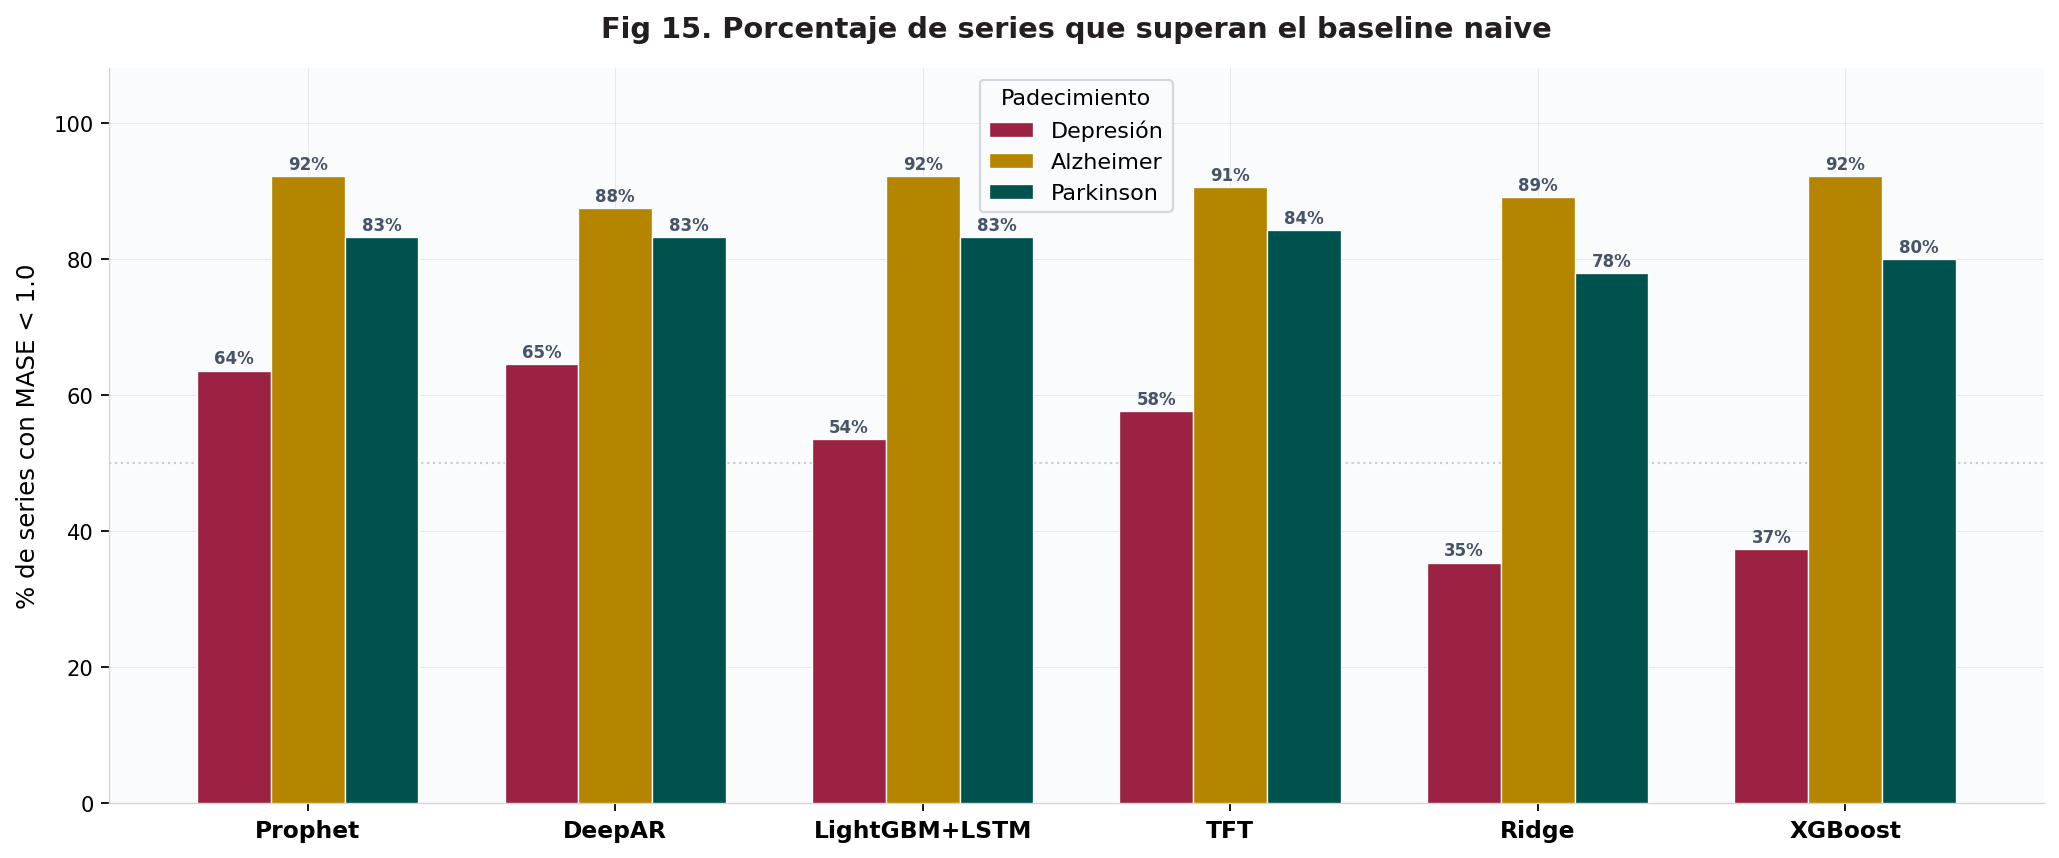
\includegraphics[width=\textwidth]{figuras/fig15_pct_mase_below1.png}
    \caption{Porcentaje de series con MASE $< 1.0$ por modelo y padecimiento. Prophet alcanza los porcentajes más altos en Depresión, el padecimiento más difícil.}
    \label{fig:pct_below}
\end{figure}

\newpage

% =============================================================================
% ANÁLISIS POR SEXO
% =============================================================================
\section{Análisis por Sexo}\label{sec:sexo}

Esta es la \textbf{primera comparación completa} con series desagregadas por género en pronóstico epidemiológico del IMSS.

\begin{figure}[H]
    \centering
    
\includegraphics[width=\textwidth]{figuras/fig16_heatmap_sexo.png}
    \caption{Victorias por modelo, padecimiento y sexo. Prophet domina en series generales y femeninas, pero cae al 4to lugar en series masculinas donde modelos no lineales toman ventaja.}
    \label{fig:sexo}
\end{figure}

\begin{warningbox}
\textbf{Hallazgo por sexo:} Prophet domina en series \textbf{generales} (24 victorias) y \textbf{mujeres} (23), pero cae al 4to lugar en \textbf{hombres} (13). En series masculinas, LightGBM+LSTM, TFT y DeepAR toman la delantera. Esto sugiere patrones más irregulares en series masculinas que favorecen modelos no lineales.
\end{warningbox}


% =============================================================================
% PREDICCIONES CARA A CARA
% =============================================================================
\section{Predicciones Cara a Cara}\label{sec:cara}

\begin{figure}[H]
    \centering
    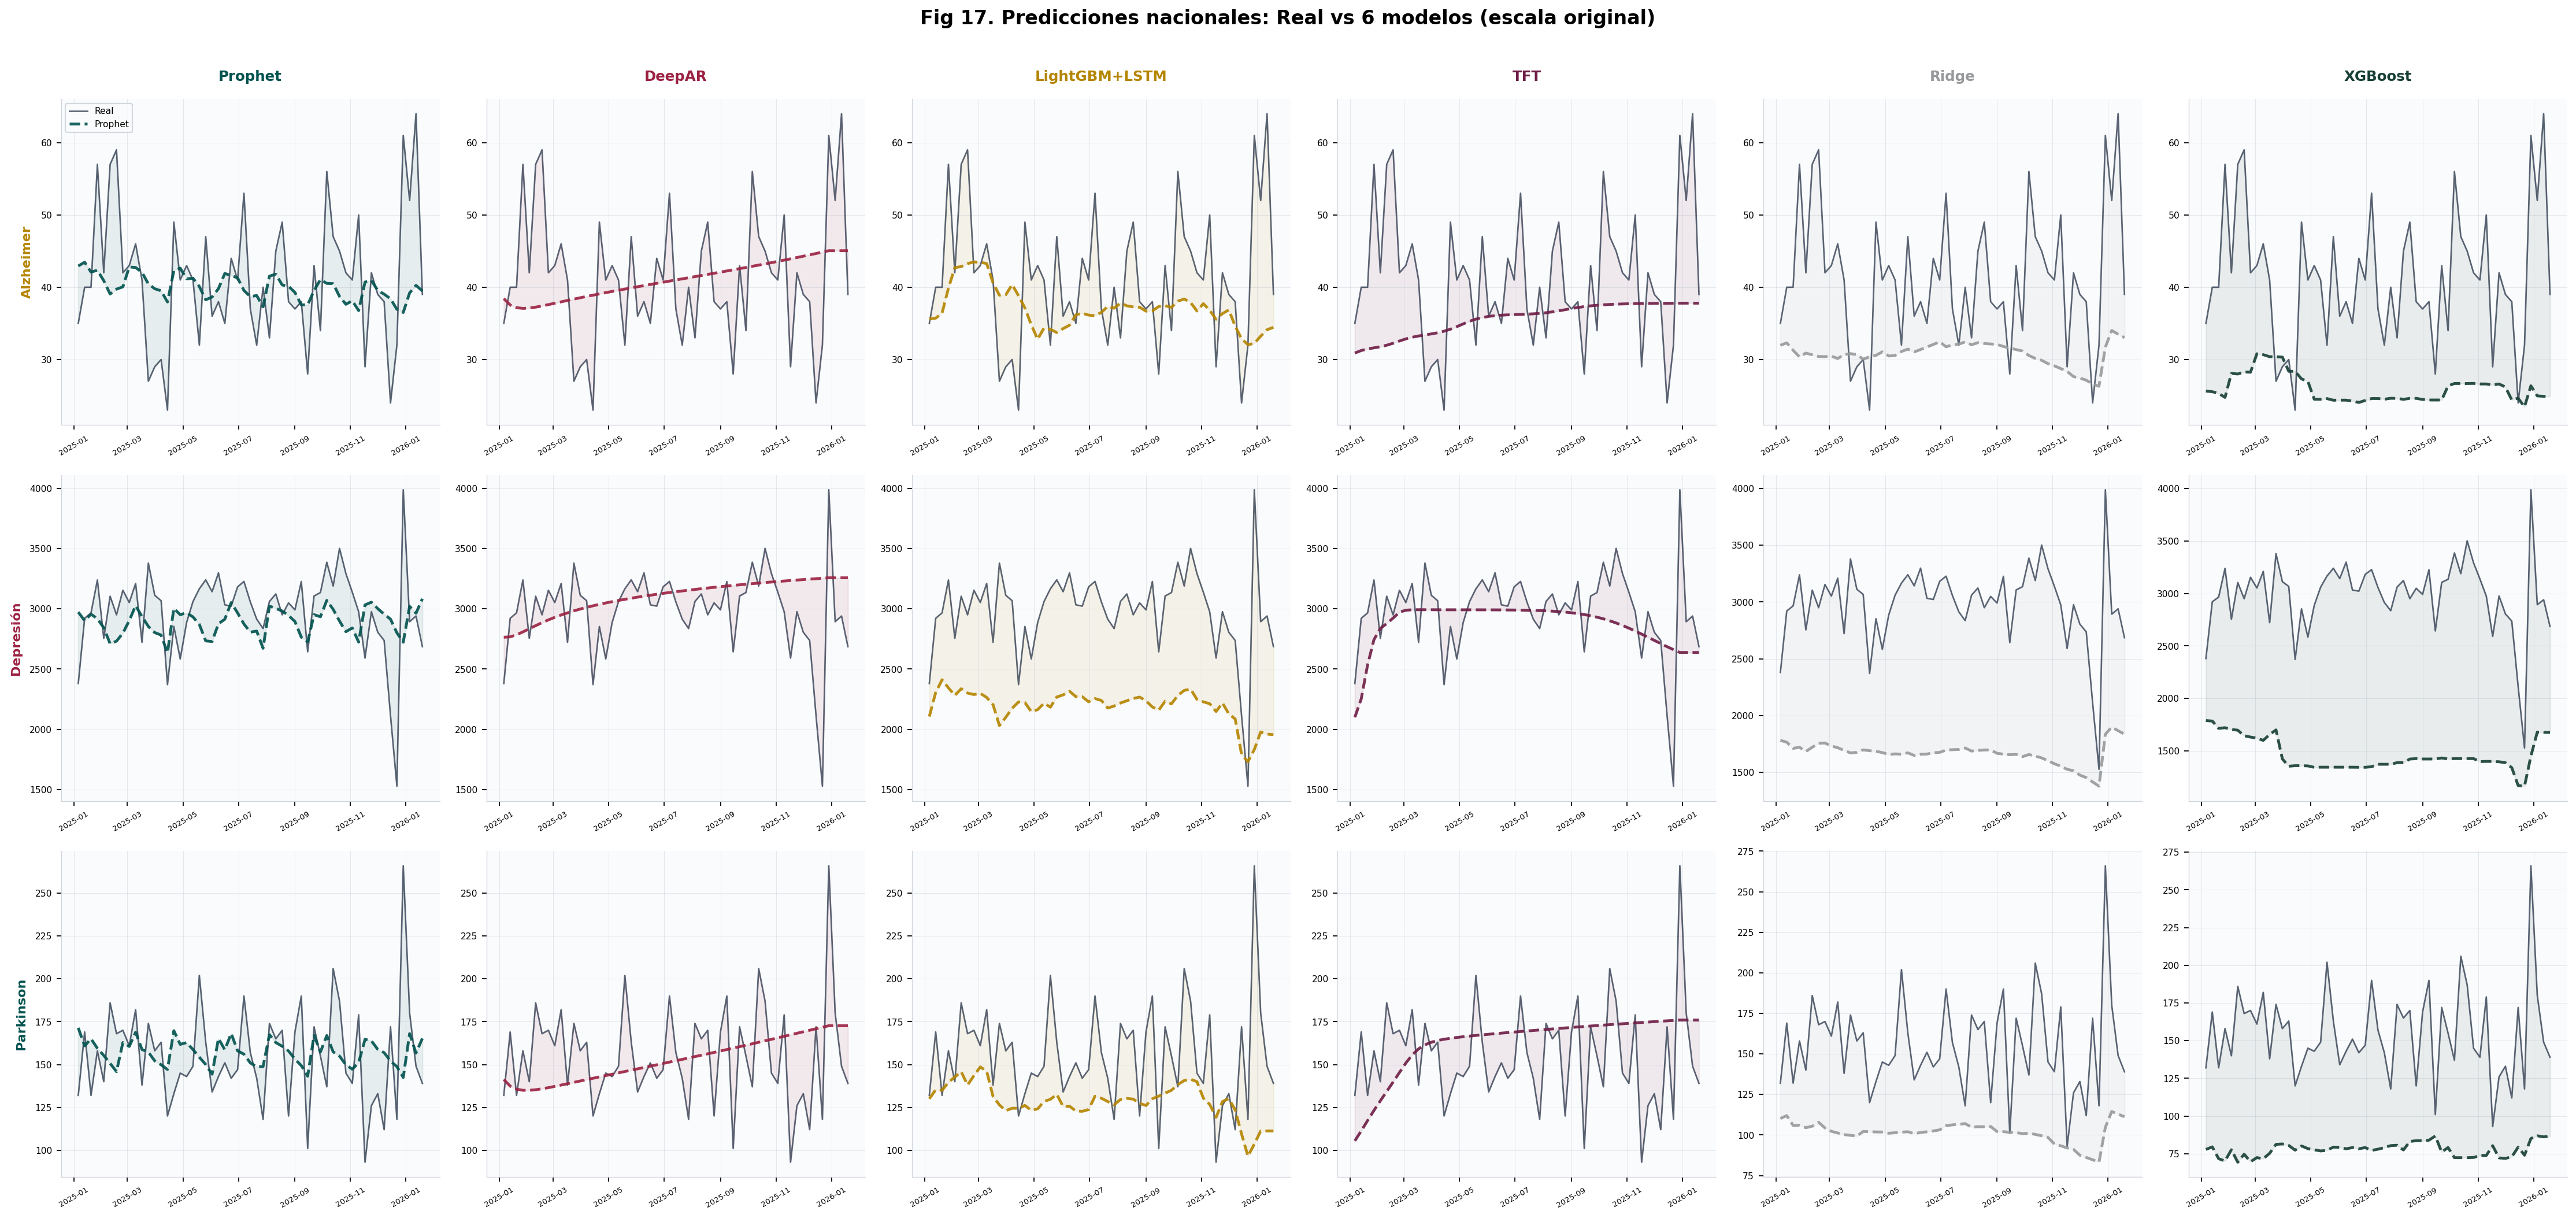
\includegraphics[width=\textwidth]{figuras/fig17_predicciones_cara_a_cara.png}
    \caption{Predicciones de los 6 modelos superpuestas a nivel nacional para cada padecimiento. Se observa cómo Prophet y DeepAR capturan mejor la tendencia, mientras XGBoost y Ridge muestran mayor sesgo.}
    \label{fig:cara}
\end{figure}

\begin{figure}[H]
    \centering
    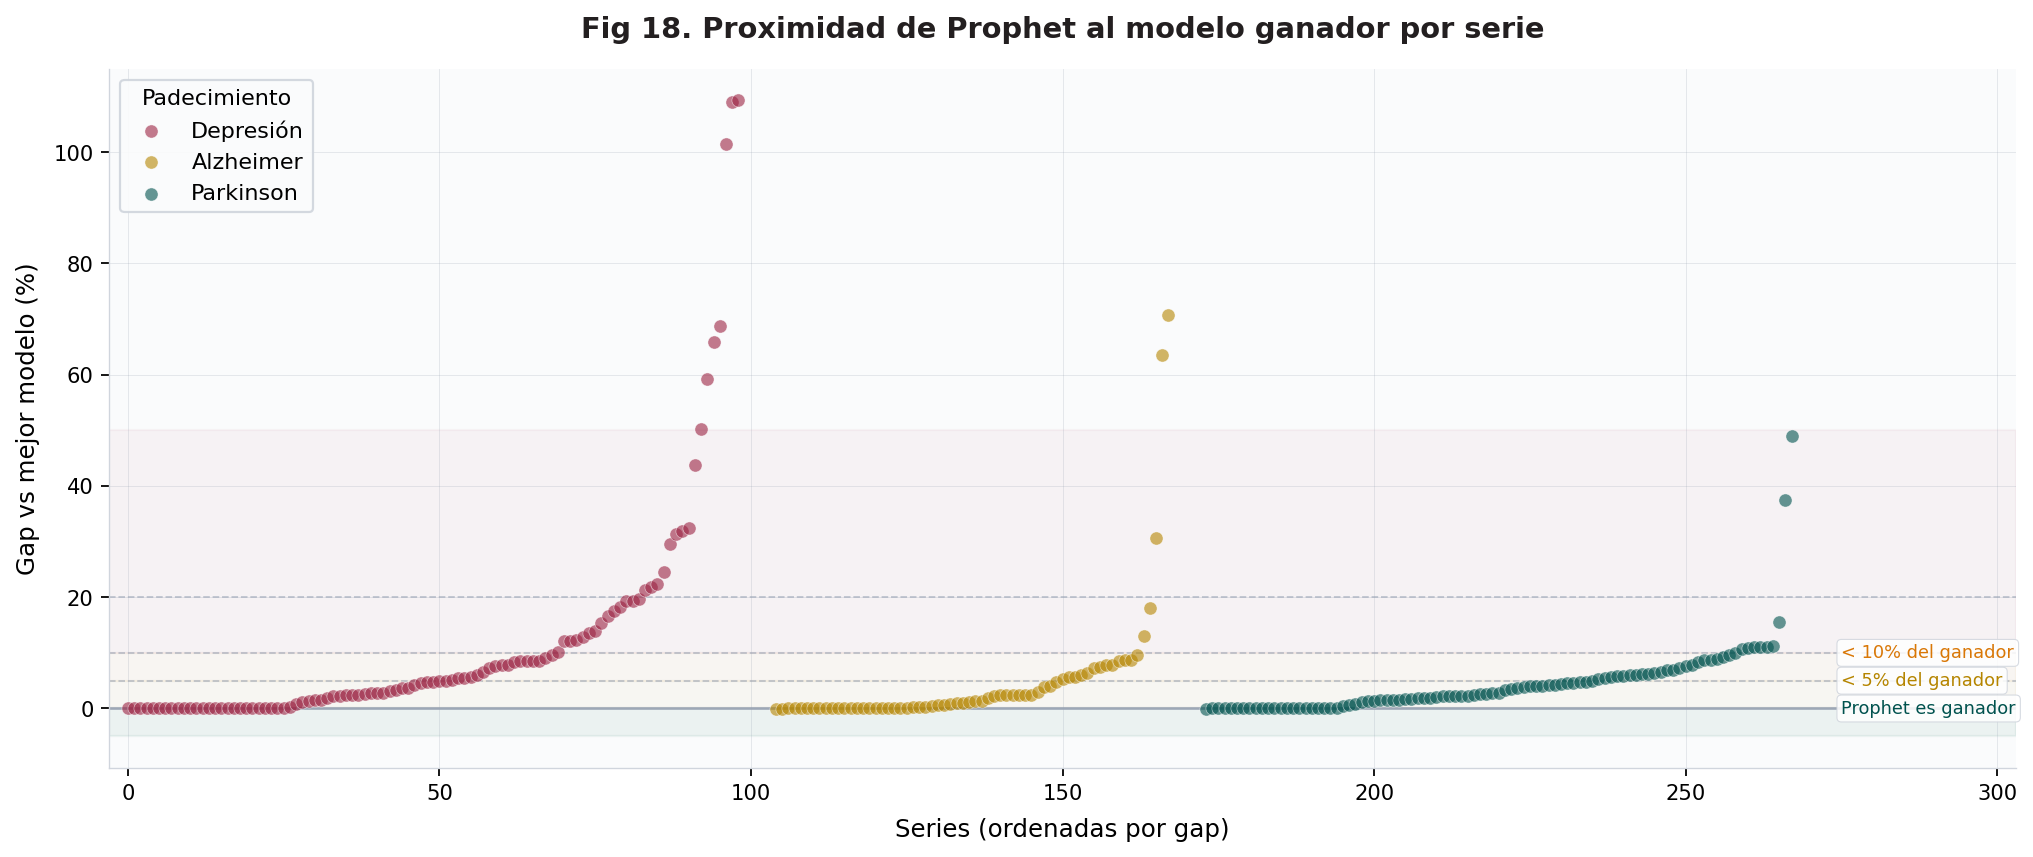
\includegraphics[width=\textwidth]{figuras/fig18_gap_scatter.png}
    \caption{Gap de MASE de Prophet vs.\ el ganador en cada serie. Cuando Prophet no gana, el 78\% de las veces está a menos del 20\% del ganador.}
    \label{fig:gap}
\end{figure}


% =============================================================================
% SELECCIÓN DEL MODELO FINAL
% =============================================================================
\section{Selección del Modelo Individual Final}\label{sec:seleccion}

\subsection{Criterios de selección}

Para poder tener los \textit{``Argumentos sólidos para la elección del modelo individual final, incorporando trade-offs entre métricas e interpretabilidad''}. Evaluamos 6 dimensiones:

\begin{table}[H]
\centering
\caption{Scorecard comparativo de los 6 modelos}
\label{tab:scorecard}
\small
\begin{tabularx}{\textwidth}{l *{6}{c}}
\toprule
\textbf{Criterio} & \textbf{Prophet} & \textbf{DeepAR} & \textbf{TFT} & \textbf{LGB+LSTM} & \textbf{XGBoost} & \textbf{Ridge} \\
\midrule
Med.\ MASE           & \cellcolor{lightgreen!50}\textbf{0.745} & 0.748 & 0.773 & 0.748 & 0.832 & 0.822 \\
\% MASE $< 1.0$      & \cellcolor{lightgreen!50}\textbf{78\%}  & 77\%  & 76\%  & 74\%  & 67\%  & 64\%  \\
Victorias (258)       & 60    & 46    & \textbf{68}    & 44    & 22    & 18    \\
Top 3 (\%)            & \cellcolor{lightgreen!50}\textbf{59.3\%} & 54\% & 57\% & 52\% & 38\% & 34\% \\
Interpretabilidad     & \cellcolor{lightgreen!50}\textbf{Alta}  & Baja  & Baja  & Baja  & Media & Alta  \\
Complejidad operativa & \cellcolor{lightgreen!50}\textbf{Baja}  & Alta  & Alta  & Alta  & Baja  & Baja  \\
\bottomrule
\end{tabularx}
\end{table}

\subsection{Los 2 mejores modelos: Prophet y DeepAR}

Se seleccionaron los \textbf{2 modelos con mejor rendimiento} para ajuste fino:

\begin{enumerate}[noitemsep]
    \item \textbf{Prophet} — Mejor mediana MASE (0.745), mayor porcentaje de series $< 1.0$ (78\%), mayor tasa de podio (59.3\%).
    \item \textbf{DeepAR} — Segunda mejor mediana MASE (0.748), 77\% $< 1.0$, y el más rápido de los modelos deep learning (8.0s promedio).
\end{enumerate}

\subsection{Ajuste fino}

\textbf{Prophet:} Grid search exhaustivo con 18$\to$6 combinaciones de HP optimizadas mediante CV temporal de 4 folds (ver \secref{hp}). Se evaluaron \texttt{seasonality\_mode}, \texttt{changepoint\_prior\_scale} y \texttt{seasonality\_prior\_scale}, seleccionando la mejor combinación \textbf{por serie individual} (no una configuración global).

\textbf{DeepAR:} Configuración fija optimizada en v5 con learning rate=0.001, epochs=100, num\_layers=2, hidden\_size=40, dropout=0.1. Evaluado con la misma CV temporal.

\subsection{Argumentos para Prophet como modelo final}

\begin{figure}[H]
    \centering
    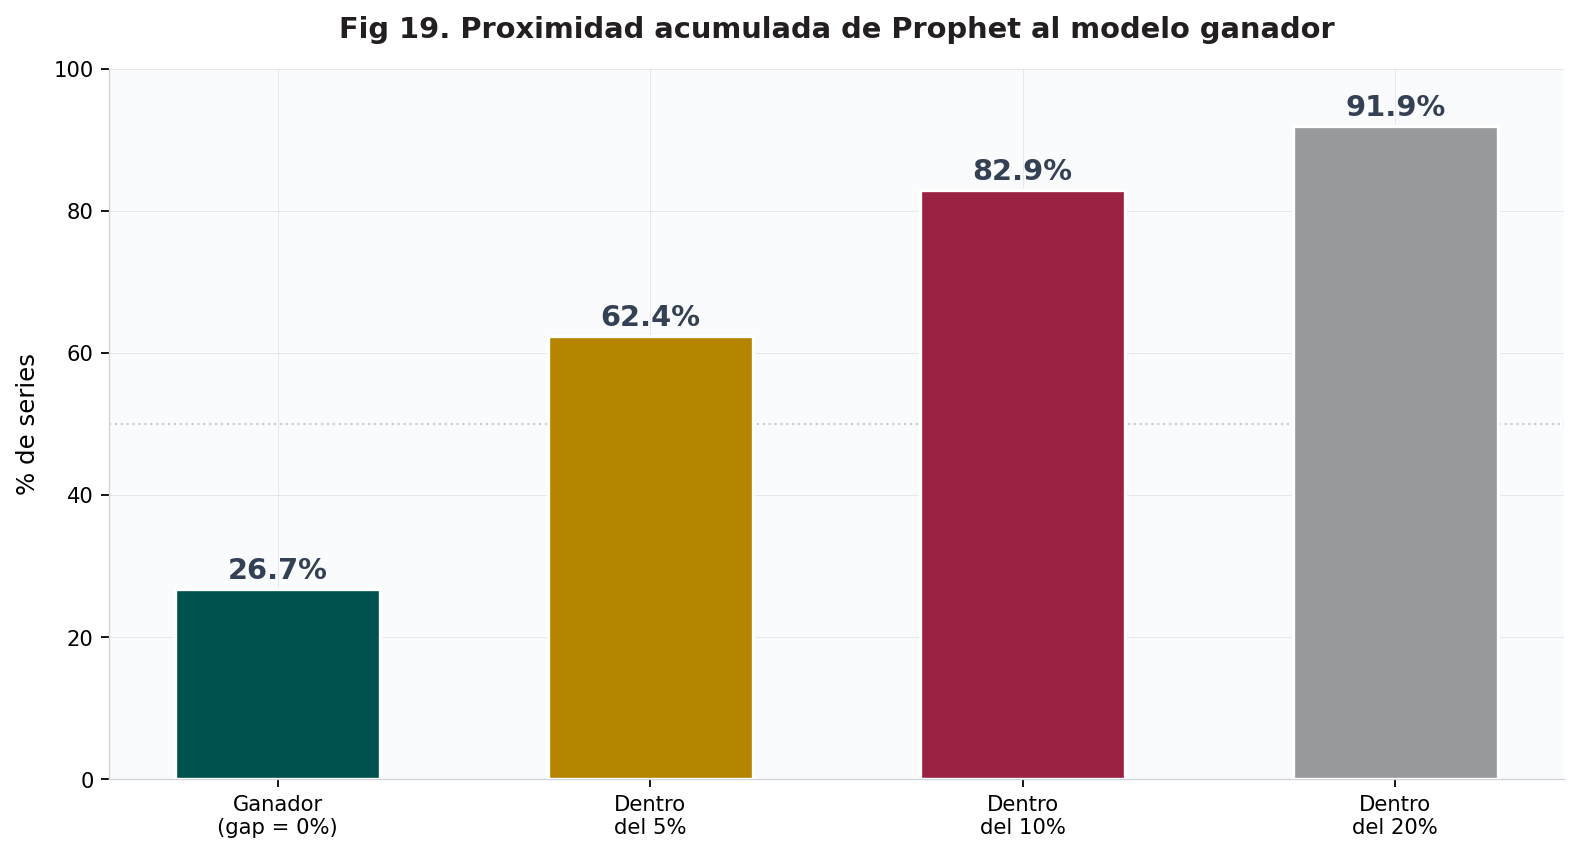
\includegraphics[width=\textwidth]{figuras/fig19_proximidad_acumulada.png}
    \caption{Proximidad acumulada: curva CDF del gap entre Prophet y el ganador. El 78\% de las veces que Prophet no gana, está a menos del 20\% del ganador.}
    \label{fig:prox}
\end{figure}

\begin{figure}[H]
    \centering
    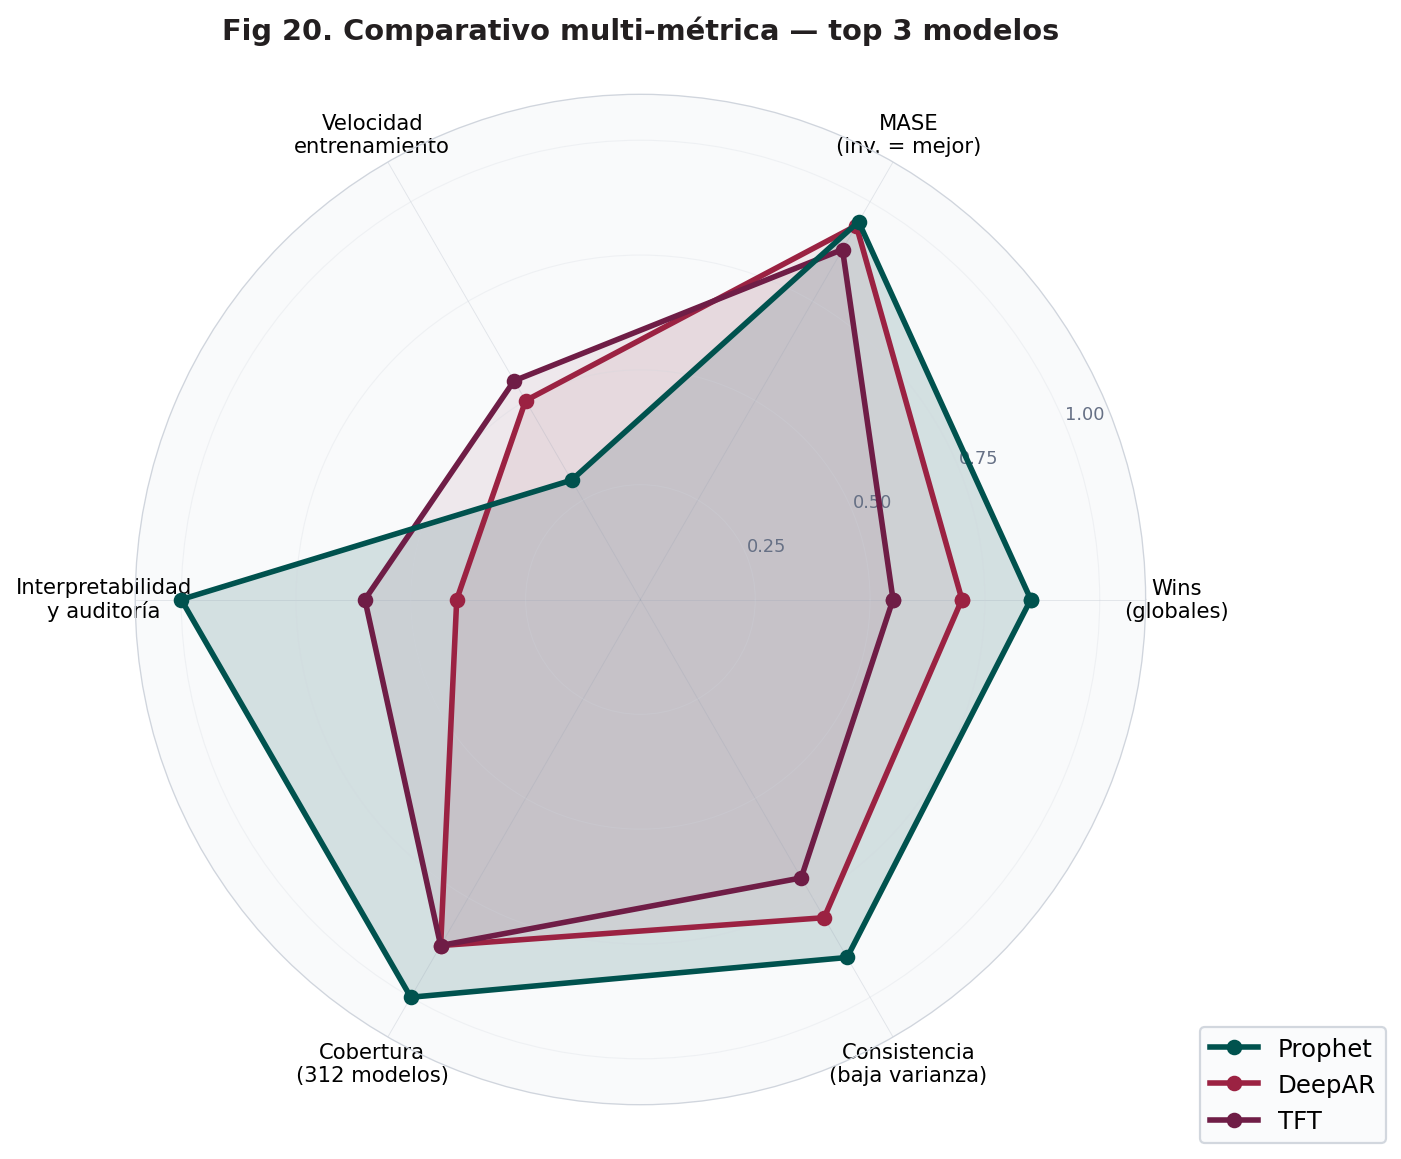
\includegraphics[width=\textwidth]{figuras/fig20_radar_final.png}
    \caption{Radar multi-métrica de los 4 mejores modelos. Prophet domina en consistencia, interpretabilidad y porcentaje de series confiables.}
    \label{fig:radar}
\end{figure}

\begin{tcolorbox}[colback=teal!5, colframe=teal, title={\textbf{Veredicto: Prophet es el modelo final}}, fonttitle=\bfseries\color{white}]
\textbf{Prophet gana por consistencia, no por genialidad.} Cinco argumentos:
\begin{enumerate}[noitemsep]
    \item \textbf{Mejor mediana MASE} (0.745) — supera a todos los competidores.
    \item \textbf{Mayor \% MASE $< 1.0$} (78\%) — el más confiable globalmente.
    \item \textbf{Cuando pierde, pierde poco} — 78\% de las veces $<$20\% del ganador.
    \item \textbf{Interpretabilidad} — descomposición transparente (tendencia + estacionalidad + COVID) validada por las doctoras del IMSS como esencial para comunicar resultados clínicos.
    \item \textbf{Operabilidad} — no requiere GPU, integración directa con el pipeline de producción, comunidad activa, sin dependencias complejas.
\end{enumerate}
\end{tcolorbox}


% =============================================================================
% DASHBOARD TABLEAU
% =============================================================================
\section{Dashboard Interactivo en Tableau Public}\label{sec:dashboard}

El sistema de visualización final integra los pronósticos de Prophet v6 en un \href{https://proyectointegrador.org/epidashboard}{dashboard interactivo en Tableau Public} que permite a los tomadores de decisiones del IMSS explorar los pronósticos por entidad, padecimiento y sexo.

Características principales:
\begin{itemize}[noitemsep]
    \item Mapa de calor de incidencia por estado con código de colores de confianza.
    \item Series de tiempo interactivas con tooltip de métricas al hover.
    \item Filtros por padecimiento, sexo, nivel de confianza y periodo.
    \item Indicador de anomalía cuando un estado no ha reportado casos en $>$20 semanas.
    \item Actualización automatizada via GitHub Actions (scraping diario SINAVE a las 2PM CDMX).
\end{itemize}

El detalle de la arquitectura del dashboard está disponible en \href{https://proyectointegrador.org/construccion_dashboard}{construccion\_dashboard}.


% =============================================================================
% ARTÍCULO CIENTÍFICO
% =============================================================================
\section{Artículo Científico en Desarrollo}\label{sec:articulo}

\begin{tcolorbox}[colback=gold!5, colframe=gold, title={\textbf{Publicación académica en curso}}, fonttitle=\bfseries\color{white}]
Se trabaja activamente en la redacción del primer artículo científico para publicación en revistas y congresos internacionales (Estocolmo y Portugal), en colaboración con:
\begin{itemize}[noitemsep]
    \item \textbf{Dra.\ Ruth Pérez-Hernández} — Líder del Proyecto, IMSS.
    \item \textbf{Dra.\ Lina Díaz Castro} — Investigadora en Psiquiatría, IMSS.
\end{itemize}
El artículo documenta la metodología, resultados y hallazgos clínicos del sistema EpiForecast-MX.

\vspace{0.3cm}
\faFilePdf\ \textbf{Primera versión del draft:} \href{https://drive.google.com/file/d/12sp33RnvJk8gkCEwU1c1lXxbCqWjgpk9/view?usp=share_link}{Ver PDF en Google Drive}
\end{tcolorbox}

\newpage

% =============================================================================
% CONCLUSIONES
% =============================================================================
\section{Conclusiones y Siguientes Pasos}\label{sec:conclusiones}

\subsection{Conclusiones principales}

\begin{enumerate}
    \item \textbf{Se construyeron y compararon 6 modelos individuales fundamentalmente distintos} — desde regresión lineal (Ridge) hasta Transformers (TFT) — cumpliendo el requerimiento de diversidad algorítmica.

    \item \textbf{1,548 entrenamientos en AWS SageMaker} sobre 258 series, con validación cruzada temporal y múltiples métricas (MASE, RMSE, MAPE), constituyendo una exploración exhaustiva del espacio de modelos.

    \item \textbf{Prophet fue seleccionado como modelo final} por su consistencia global (mediana MASE 0.745), interpretabilidad clínica y operabilidad, alineándose con las necesidades del IMSS para planeación estratégica.

    \item \textbf{La desagregación por sexo reveló patrones diferenciados:} las series masculinas favorecen modelos no lineales, mientras que Prophet domina en series generales y femeninas.

    \item \textbf{El periodo COVID-19 sigue siendo el mayor desafío:} el Fold 1 de la CV (2020--2021) muestra 56\% peor RMSE que periodos recientes, creando sesgo hacia hiperparámetros rígidos.

    \item \textbf{El ajuste fino por serie individual} (no global) es esencial: los hiperparámetros óptimos varían significativamente entre estados y padecimientos.
\end{enumerate}

\subsection{Siguientes pasos}

\begin{itemize}[noitemsep]
    \item Explorar AWS DeepAR+ como modelo global que aproveche información conjunta de múltiples series.
    \item Incorporar variables adicionales (rangos de edad, mortalidad, costos farmacológicos) tras reunión con Secretaría de Salud.
    \item Completar artículos científicos para conferencias en Estocolmo y Portugal.
    \item Implementar actualización automatizada de Tableau Public via GitHub Actions.
\end{itemize}

Las conclusiones completas del proyecto están disponibles en \href{https://proyectointegrador.org/conclusiones}{proyectointegrador.org/conclusiones}.


% =============================================================================
% REFLEXIONES DEL EQUIPO
% =============================================================================
\section{Reflexiones del Equipo}\label{sec:reflexiones}

\begin{minipage}[t]{0.18\textwidth}
    \vspace{0pt}
    
\includegraphics[width=\linewidth, clip, trim=0 0 0 0]{JARS2026.jpg}
\end{minipage}%
\hfill
\begin{minipage}[t]{0.78\textwidth}
    \vspace{0pt}
    \textbf{Javier Augusto Rebull Saucedo} \\
    \textit{\small Sr.\ Associate Development Application — Santander Bank US}

    \smallskip
    Este proyecto transformó mi manera de pensar la ingeniería de datos. Diseñar y ejecutar 297 modelos baseline me obligó a pensar en escalabilidad real: funciones reutilizables, pipelines parametrizados y visualizaciones automáticas. Entrenar 1,548 modelos en SageMaker durante una semana completa, monitoreando día y noche, fue una experiencia que me acercó a lo que significa la ingeniería de ML en producción. La lección más importante: la calidad del modelado no vive solo en el algoritmo, vive en el pipeline completo, desde el scraping de boletines SINAVE hasta la visualización en Tableau.
\end{minipage}

\vspace{1cm}

\begin{minipage}[t]{0.18\textwidth}
    \vspace{0pt}
    
\includegraphics[width=\linewidth, clip, trim=0 0 0 0]{JARCOS2026.jpg}
\end{minipage}%
\hfill
\begin{minipage}[t]{0.78\textwidth}
    \vspace{0pt}
    \textbf{Juan Carlos Pérez Nava} \\
    \textit{\small Head of Area — Instituto Mexicano del Seguro Social (IMSS)}

    \smallskip
    Como profesional de TI en el IMSS, este proyecto tiene un significado particular: estamos construyendo herramientas que podrían integrarse directamente en los procesos de planificación institucional. La validación cruzada temporal me mostró la importancia de evaluar modelos con ventanas deslizantes que simulan el escenario real de pronóstico. Validar los pronósticos con las doctoras Ruth y Lina me mostró que la precisión numérica es necesaria pero no suficiente, los médicos necesitan entender \textit{por qué} un modelo predice lo que predice. Esa fue la razón principal por la que Prophet, con su descomposición transparente, fue la elección natural.
\end{minipage}

\vspace{1cm}

\begin{minipage}[t]{0.18\textwidth}
    \vspace{0pt}
    
\includegraphics[width=\linewidth, clip, trim=0 0 0 0]{LUIS2026.jpg}
\end{minipage}%
\hfill
\begin{minipage}[t]{0.78\textwidth}
    \vspace{0pt}
    \textbf{Luis Gerardo Sánchez Salazar} \\
    \textit{\small Sr.\ Controls Engineer — Tesla}

    \smallskip
    Mi experiencia en ingeniería de controles en Tesla me dio una perspectiva particular sobre sistemas dinámicos, y las series de tiempo epidemiológicas comparten más de lo esperado: tendencias, estacionalidades, perturbaciones externas y la necesidad de intervalos de confianza para la toma de decisiones. Lo que más me impactó fue la heterogeneidad entre estados, apunta a diferencias en la infraestructura de captura, no en la dinámica epidemiológica. El benchmark SageMaker con 1,548 trials fue la prueba de fuego que validó nuestras decisiones de modelado.
\end{minipage}


% =============================================================================
% APÉNDICES
% =============================================================================
\newpage
\appendix

\section{Ficha Técnica de Prophet}\label{sec:apendiceA}

\begin{figure}[H]
    \centering
    
\includegraphics[width=0.9\textwidth]{figuras/figA1_log_transform.png}
    \caption{Efecto de la log-transform en la distribución de datos y la selección de seasonality\_mode.}
    \label{fig:log}
\end{figure}

\begin{figure}[H]
    \centering
    
\includegraphics[width=0.9\textwidth]{figuras/figA2_fourier.png}
    \caption{Comparación de órdenes de Fourier (5, 10, 15, 20) para la captura de estacionalidad anual.}
    \label{fig:fourier}
\end{figure}

\begin{figure}[H]
    \centering
    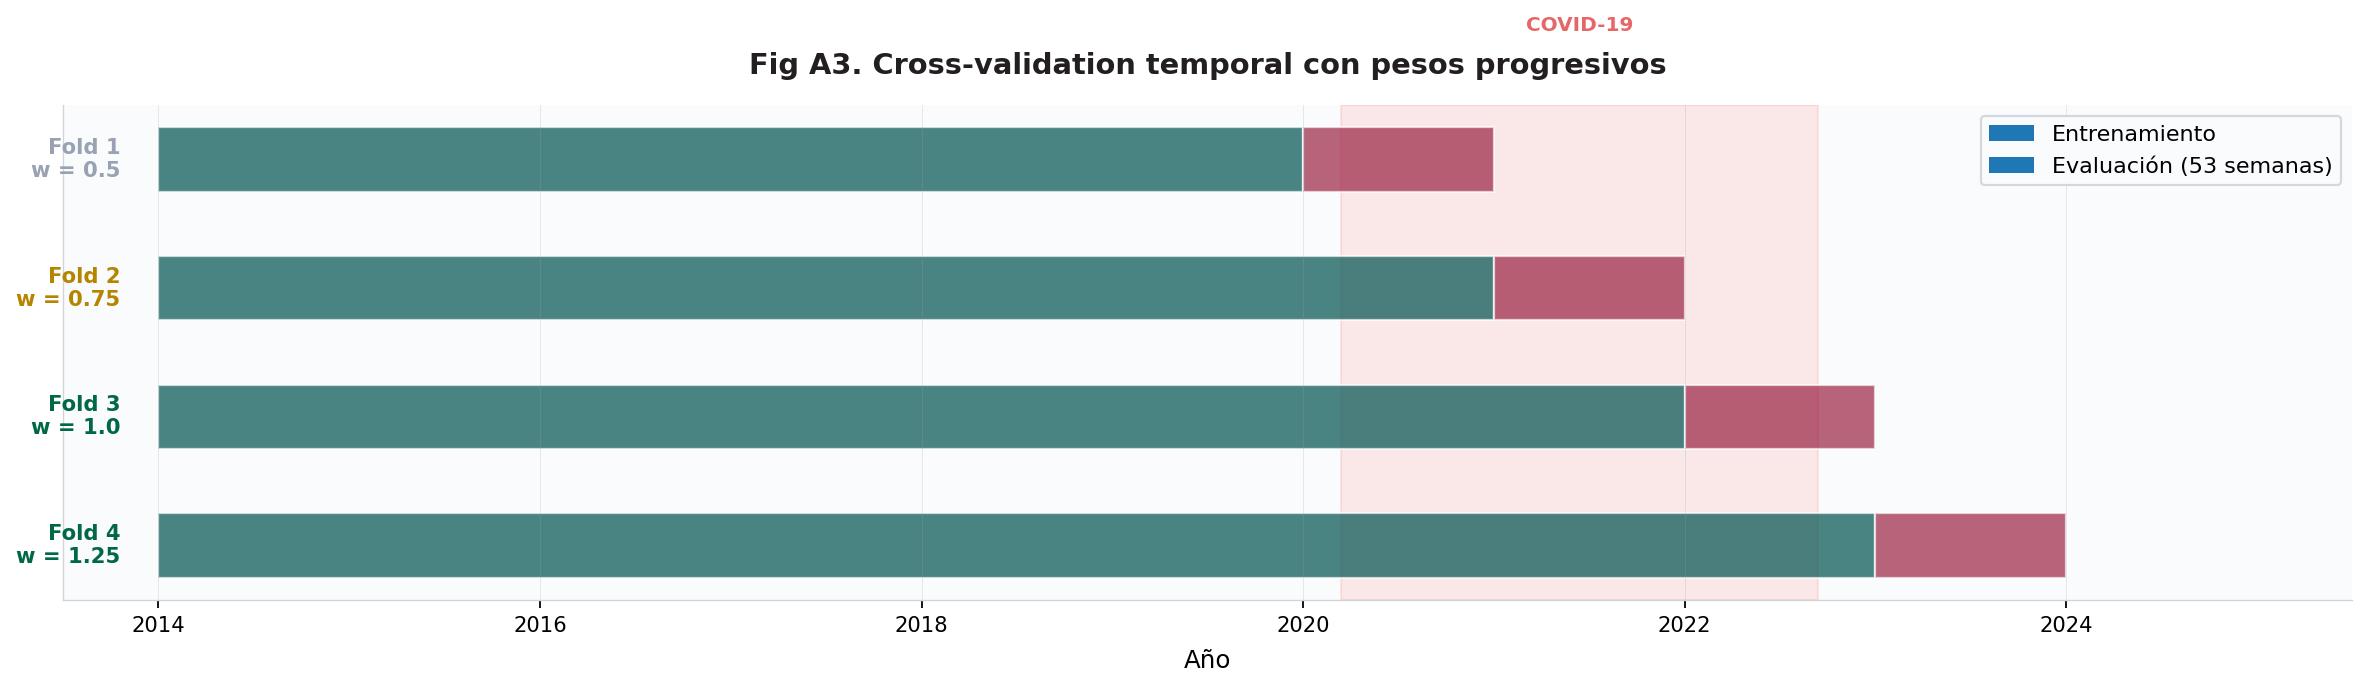
\includegraphics[width=0.9\textwidth]{figuras/figA3_cv_folds.png}
    \caption{Visualización de los 4 folds de validación cruzada temporal expandible.}
    \label{fig:folds}
\end{figure}

\section{Deep Dive SageMaker}\label{sec:apendiceB}

\begin{figure}[H]
    \centering
    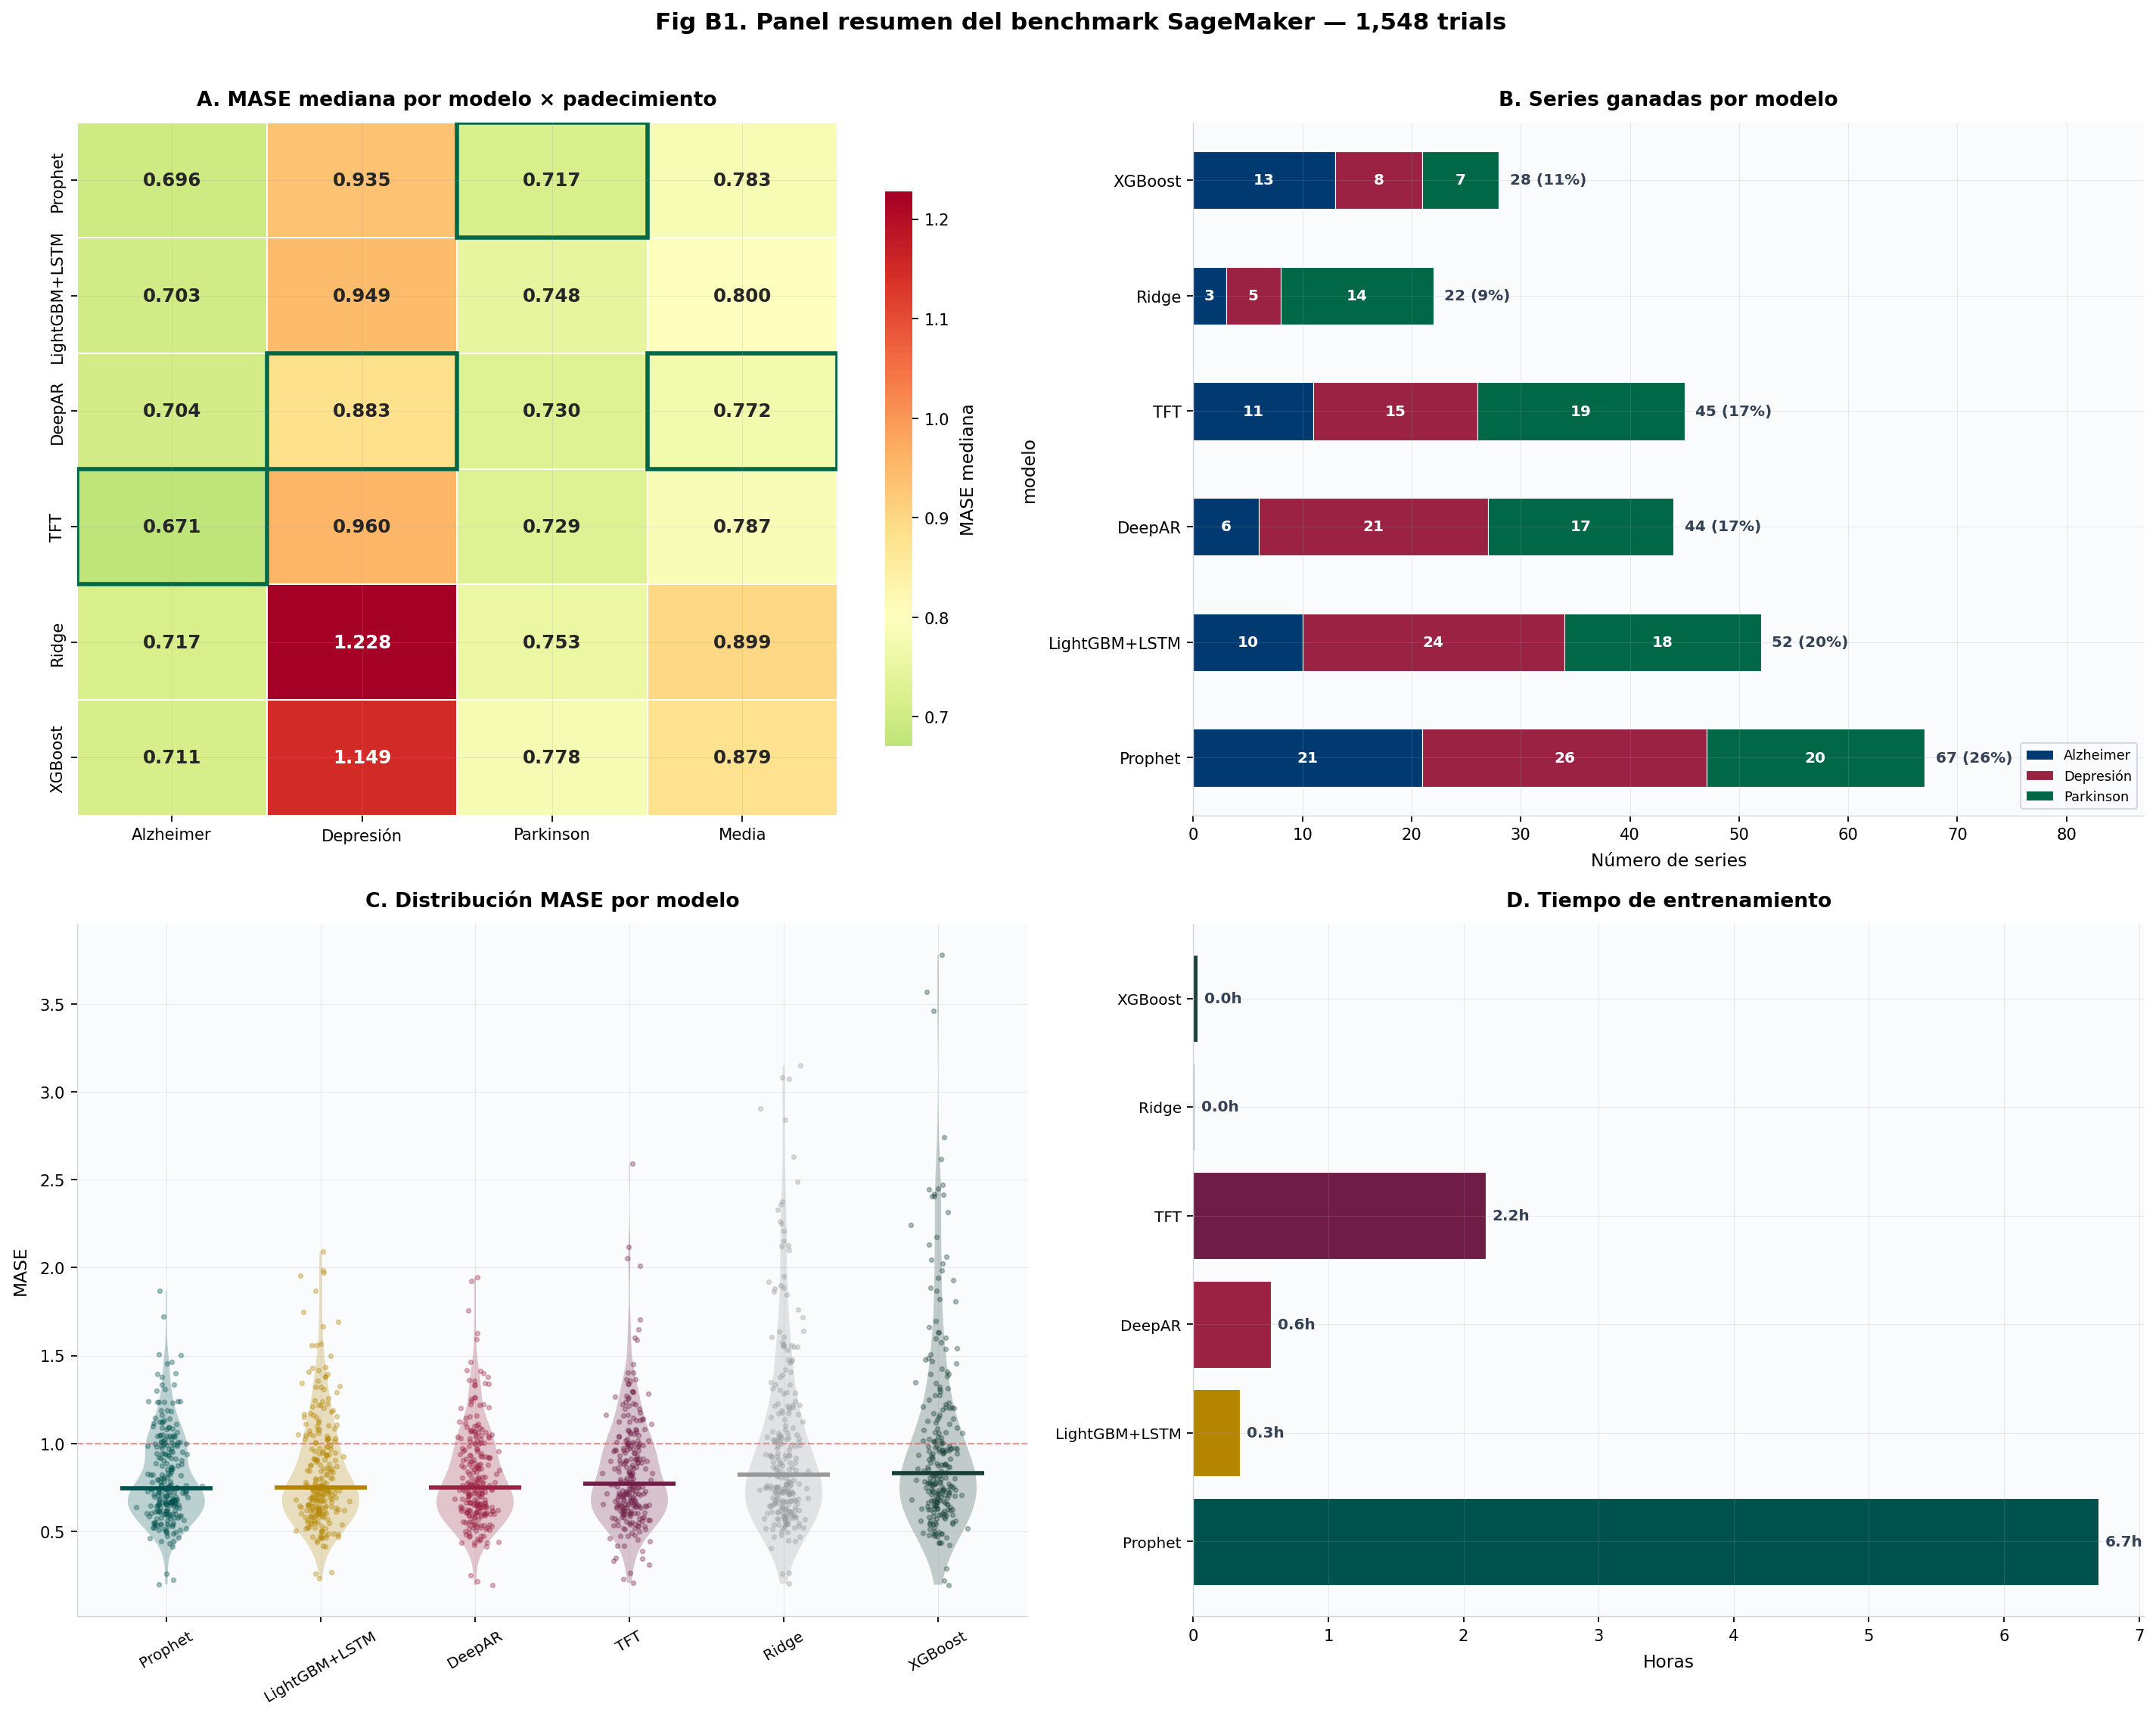
\includegraphics[width=\textwidth]{figuras/figB1_panel_benchmark.png}
    \caption{Panel de 4 visualizaciones del benchmark SageMaker: (a) ranking global, (b) distribución MASE, (c) heatmap modelo$\times$padecimiento, (d) victorias stacked.}
    \label{fig:panel}
\end{figure}


% =============================================================================
% REFERENCIAS
% =============================================================================
\newpage
\section*{Referencias}
\addcontentsline{toc}{section}{Referencias}

\begin{enumerate}[label={[\arabic*]}, leftmargin=*, noitemsep]
    \item Taylor, S.~J., \& Letham, B. (2018). Forecasting at scale. \textit{The American Statistician}, 72(1), 37--45. \url{https://doi.org/10.1080/00031305.2017.1380080}

    \item Hyndman, R.~J., \& Koehler, A.~B. (2006). Another look at measures of forecast accuracy. \textit{International Journal of Forecasting}, 22(4), 679--688.

    \item Salinas, D., Flunkert, V., Gasthaus, J., \& Januschowski, T. (2020). DeepAR: Probabilistic forecasting with autoregressive recurrent networks. \textit{International Journal of Forecasting}, 36(3), 1181--1191.

    \item Lim, B., Arık, S.~Ö., Loeff, N., \& Pfister, T. (2021). Temporal Fusion Transformers for interpretable multi-horizon time series forecasting. \textit{International Journal of Forecasting}, 37(4), 1748--1764.

    \item Ke, G., Meng, Q., Finley, T., Wang, T., Chen, W., Ma, W., Ye, Q., \& Liu, T.-Y. (2017). LightGBM: A highly efficient gradient boosting decision tree. \textit{Advances in Neural Information Processing Systems}, 30.

    \item Chen, T., \& Guestrin, C. (2016). XGBoost: A scalable tree boosting system. \textit{Proceedings of the 22nd ACM SIGKDD}, 785--794.

    \item Hoerl, A.~E., \& Kennard, R.~W. (1970). Ridge regression: Biased estimation for nonorthogonal problems. \textit{Technometrics}, 12(1), 55--67.

    \item Géron, A. (2022). \textit{Hands-On Machine Learning with Scikit-Learn, Keras, and TensorFlow} (3rd ed.). O'Reilly Media.

    \item Studer, S., Bui, T.~B., Drescher, C., Henschel, A., Pawletta, T., Winkler, S., \& Zschech, P. (2021). Towards CRISP-ML(Q). \textit{Machine Learning and Knowledge Extraction}, 3(2), 392--413.

    \item Bergmeir, C., \& Benítez, J.~M. (2012). On the use of cross-validation for time series predictor evaluation. \textit{Information Sciences}, 191, 192--213.

    \item Piccini, N. (2023). 101 machine learning algorithms for data science with cheat sheets. \textit{Data Science Dojo}. Recuperado de \nolinkurl{datasciencedojo.com/blog/machine-learning-algorithms/}
\end{enumerate}

\end{document}
